% Generated by Sphinx.
\def\sphinxdocclass{report}
\documentclass[letterpaper,10pt,english]{sphinxmanual}
\usepackage[utf8]{inputenc}
\DeclareUnicodeCharacter{00A0}{\nobreakspace}
\usepackage{cmap}
\usepackage[T1]{fontenc}
\usepackage{babel}
\usepackage{times}
\usepackage[Bjarne]{fncychap}
\usepackage{longtable}
\usepackage{sphinx}
\usepackage{multirow}

\usepackage{fontspec}     % 引入 fontsepc,這樣才可以用下面的設定字型的指令
\setmainfont{AR PL UKai TW}  % 預設字型
\setsansfont{AR PL UKai TW}  % sans family 字型
\setromanfont{AR PL UKai TW} % roman 字型
\setmonofont{AR PL UKai TW}  % 等寬字型

\XeTeXlinebreaklocale "zh"          % 設定斷行演算法為中文
\XeTeXlinebreakskip = 0pt plus 1pt  % 設定中文字距與英文字距


\title{系統安裝記錄 Documentation}
\date{October 21, 2014}
\release{1.0}
\author{陳國華}
\newcommand{\sphinxlogo}{}
\renewcommand{\releasename}{Release}
\makeindex

\makeatletter
\def\PYG@reset{\let\PYG@it=\relax \let\PYG@bf=\relax%
    \let\PYG@ul=\relax \let\PYG@tc=\relax%
    \let\PYG@bc=\relax \let\PYG@ff=\relax}
\def\PYG@tok#1{\csname PYG@tok@#1\endcsname}
\def\PYG@toks#1+{\ifx\relax#1\empty\else%
    \PYG@tok{#1}\expandafter\PYG@toks\fi}
\def\PYG@do#1{\PYG@bc{\PYG@tc{\PYG@ul{%
    \PYG@it{\PYG@bf{\PYG@ff{#1}}}}}}}
\def\PYG#1#2{\PYG@reset\PYG@toks#1+\relax+\PYG@do{#2}}

\expandafter\def\csname PYG@tok@si\endcsname{\let\PYG@it=\textit\def\PYG@tc##1{\textcolor[rgb]{0.44,0.63,0.82}{##1}}}
\expandafter\def\csname PYG@tok@mh\endcsname{\def\PYG@tc##1{\textcolor[rgb]{0.13,0.50,0.31}{##1}}}
\expandafter\def\csname PYG@tok@vc\endcsname{\def\PYG@tc##1{\textcolor[rgb]{0.73,0.38,0.84}{##1}}}
\expandafter\def\csname PYG@tok@na\endcsname{\def\PYG@tc##1{\textcolor[rgb]{0.25,0.44,0.63}{##1}}}
\expandafter\def\csname PYG@tok@mi\endcsname{\def\PYG@tc##1{\textcolor[rgb]{0.13,0.50,0.31}{##1}}}
\expandafter\def\csname PYG@tok@vi\endcsname{\def\PYG@tc##1{\textcolor[rgb]{0.73,0.38,0.84}{##1}}}
\expandafter\def\csname PYG@tok@nn\endcsname{\let\PYG@bf=\textbf\def\PYG@tc##1{\textcolor[rgb]{0.05,0.52,0.71}{##1}}}
\expandafter\def\csname PYG@tok@sc\endcsname{\def\PYG@tc##1{\textcolor[rgb]{0.25,0.44,0.63}{##1}}}
\expandafter\def\csname PYG@tok@nt\endcsname{\let\PYG@bf=\textbf\def\PYG@tc##1{\textcolor[rgb]{0.02,0.16,0.45}{##1}}}
\expandafter\def\csname PYG@tok@mo\endcsname{\def\PYG@tc##1{\textcolor[rgb]{0.13,0.50,0.31}{##1}}}
\expandafter\def\csname PYG@tok@gt\endcsname{\def\PYG@tc##1{\textcolor[rgb]{0.00,0.27,0.87}{##1}}}
\expandafter\def\csname PYG@tok@vg\endcsname{\def\PYG@tc##1{\textcolor[rgb]{0.73,0.38,0.84}{##1}}}
\expandafter\def\csname PYG@tok@kd\endcsname{\let\PYG@bf=\textbf\def\PYG@tc##1{\textcolor[rgb]{0.00,0.44,0.13}{##1}}}
\expandafter\def\csname PYG@tok@se\endcsname{\let\PYG@bf=\textbf\def\PYG@tc##1{\textcolor[rgb]{0.25,0.44,0.63}{##1}}}
\expandafter\def\csname PYG@tok@c\endcsname{\let\PYG@it=\textit\def\PYG@tc##1{\textcolor[rgb]{0.25,0.50,0.56}{##1}}}
\expandafter\def\csname PYG@tok@bp\endcsname{\def\PYG@tc##1{\textcolor[rgb]{0.00,0.44,0.13}{##1}}}
\expandafter\def\csname PYG@tok@ge\endcsname{\let\PYG@it=\textit}
\expandafter\def\csname PYG@tok@c1\endcsname{\let\PYG@it=\textit\def\PYG@tc##1{\textcolor[rgb]{0.25,0.50,0.56}{##1}}}
\expandafter\def\csname PYG@tok@gd\endcsname{\def\PYG@tc##1{\textcolor[rgb]{0.63,0.00,0.00}{##1}}}
\expandafter\def\csname PYG@tok@kn\endcsname{\let\PYG@bf=\textbf\def\PYG@tc##1{\textcolor[rgb]{0.00,0.44,0.13}{##1}}}
\expandafter\def\csname PYG@tok@ni\endcsname{\let\PYG@bf=\textbf\def\PYG@tc##1{\textcolor[rgb]{0.84,0.33,0.22}{##1}}}
\expandafter\def\csname PYG@tok@kp\endcsname{\def\PYG@tc##1{\textcolor[rgb]{0.00,0.44,0.13}{##1}}}
\expandafter\def\csname PYG@tok@w\endcsname{\def\PYG@tc##1{\textcolor[rgb]{0.73,0.73,0.73}{##1}}}
\expandafter\def\csname PYG@tok@s\endcsname{\def\PYG@tc##1{\textcolor[rgb]{0.25,0.44,0.63}{##1}}}
\expandafter\def\csname PYG@tok@gp\endcsname{\let\PYG@bf=\textbf\def\PYG@tc##1{\textcolor[rgb]{0.78,0.36,0.04}{##1}}}
\expandafter\def\csname PYG@tok@sr\endcsname{\def\PYG@tc##1{\textcolor[rgb]{0.14,0.33,0.53}{##1}}}
\expandafter\def\csname PYG@tok@mf\endcsname{\def\PYG@tc##1{\textcolor[rgb]{0.13,0.50,0.31}{##1}}}
\expandafter\def\csname PYG@tok@ne\endcsname{\def\PYG@tc##1{\textcolor[rgb]{0.00,0.44,0.13}{##1}}}
\expandafter\def\csname PYG@tok@go\endcsname{\def\PYG@tc##1{\textcolor[rgb]{0.20,0.20,0.20}{##1}}}
\expandafter\def\csname PYG@tok@sb\endcsname{\def\PYG@tc##1{\textcolor[rgb]{0.25,0.44,0.63}{##1}}}
\expandafter\def\csname PYG@tok@no\endcsname{\def\PYG@tc##1{\textcolor[rgb]{0.38,0.68,0.84}{##1}}}
\expandafter\def\csname PYG@tok@kc\endcsname{\let\PYG@bf=\textbf\def\PYG@tc##1{\textcolor[rgb]{0.00,0.44,0.13}{##1}}}
\expandafter\def\csname PYG@tok@kt\endcsname{\def\PYG@tc##1{\textcolor[rgb]{0.56,0.13,0.00}{##1}}}
\expandafter\def\csname PYG@tok@nf\endcsname{\def\PYG@tc##1{\textcolor[rgb]{0.02,0.16,0.49}{##1}}}
\expandafter\def\csname PYG@tok@gu\endcsname{\let\PYG@bf=\textbf\def\PYG@tc##1{\textcolor[rgb]{0.50,0.00,0.50}{##1}}}
\expandafter\def\csname PYG@tok@nv\endcsname{\def\PYG@tc##1{\textcolor[rgb]{0.73,0.38,0.84}{##1}}}
\expandafter\def\csname PYG@tok@gh\endcsname{\let\PYG@bf=\textbf\def\PYG@tc##1{\textcolor[rgb]{0.00,0.00,0.50}{##1}}}
\expandafter\def\csname PYG@tok@gr\endcsname{\def\PYG@tc##1{\textcolor[rgb]{1.00,0.00,0.00}{##1}}}
\expandafter\def\csname PYG@tok@il\endcsname{\def\PYG@tc##1{\textcolor[rgb]{0.13,0.50,0.31}{##1}}}
\expandafter\def\csname PYG@tok@nl\endcsname{\let\PYG@bf=\textbf\def\PYG@tc##1{\textcolor[rgb]{0.00,0.13,0.44}{##1}}}
\expandafter\def\csname PYG@tok@cs\endcsname{\def\PYG@tc##1{\textcolor[rgb]{0.25,0.50,0.56}{##1}}\def\PYG@bc##1{\setlength{\fboxsep}{0pt}\colorbox[rgb]{1.00,0.94,0.94}{\strut ##1}}}
\expandafter\def\csname PYG@tok@o\endcsname{\def\PYG@tc##1{\textcolor[rgb]{0.40,0.40,0.40}{##1}}}
\expandafter\def\csname PYG@tok@nb\endcsname{\def\PYG@tc##1{\textcolor[rgb]{0.00,0.44,0.13}{##1}}}
\expandafter\def\csname PYG@tok@cm\endcsname{\let\PYG@it=\textit\def\PYG@tc##1{\textcolor[rgb]{0.25,0.50,0.56}{##1}}}
\expandafter\def\csname PYG@tok@gs\endcsname{\let\PYG@bf=\textbf}
\expandafter\def\csname PYG@tok@s1\endcsname{\def\PYG@tc##1{\textcolor[rgb]{0.25,0.44,0.63}{##1}}}
\expandafter\def\csname PYG@tok@gi\endcsname{\def\PYG@tc##1{\textcolor[rgb]{0.00,0.63,0.00}{##1}}}
\expandafter\def\csname PYG@tok@sd\endcsname{\let\PYG@it=\textit\def\PYG@tc##1{\textcolor[rgb]{0.25,0.44,0.63}{##1}}}
\expandafter\def\csname PYG@tok@nc\endcsname{\let\PYG@bf=\textbf\def\PYG@tc##1{\textcolor[rgb]{0.05,0.52,0.71}{##1}}}
\expandafter\def\csname PYG@tok@nd\endcsname{\let\PYG@bf=\textbf\def\PYG@tc##1{\textcolor[rgb]{0.33,0.33,0.33}{##1}}}
\expandafter\def\csname PYG@tok@cp\endcsname{\def\PYG@tc##1{\textcolor[rgb]{0.00,0.44,0.13}{##1}}}
\expandafter\def\csname PYG@tok@err\endcsname{\def\PYG@bc##1{\setlength{\fboxsep}{0pt}\fcolorbox[rgb]{1.00,0.00,0.00}{1,1,1}{\strut ##1}}}
\expandafter\def\csname PYG@tok@ss\endcsname{\def\PYG@tc##1{\textcolor[rgb]{0.32,0.47,0.09}{##1}}}
\expandafter\def\csname PYG@tok@kr\endcsname{\let\PYG@bf=\textbf\def\PYG@tc##1{\textcolor[rgb]{0.00,0.44,0.13}{##1}}}
\expandafter\def\csname PYG@tok@sx\endcsname{\def\PYG@tc##1{\textcolor[rgb]{0.78,0.36,0.04}{##1}}}
\expandafter\def\csname PYG@tok@m\endcsname{\def\PYG@tc##1{\textcolor[rgb]{0.13,0.50,0.31}{##1}}}
\expandafter\def\csname PYG@tok@sh\endcsname{\def\PYG@tc##1{\textcolor[rgb]{0.25,0.44,0.63}{##1}}}
\expandafter\def\csname PYG@tok@k\endcsname{\let\PYG@bf=\textbf\def\PYG@tc##1{\textcolor[rgb]{0.00,0.44,0.13}{##1}}}
\expandafter\def\csname PYG@tok@ow\endcsname{\let\PYG@bf=\textbf\def\PYG@tc##1{\textcolor[rgb]{0.00,0.44,0.13}{##1}}}
\expandafter\def\csname PYG@tok@s2\endcsname{\def\PYG@tc##1{\textcolor[rgb]{0.25,0.44,0.63}{##1}}}

\def\PYGZbs{\char`\\}
\def\PYGZus{\char`\_}
\def\PYGZob{\char`\{}
\def\PYGZcb{\char`\}}
\def\PYGZca{\char`\^}
\def\PYGZam{\char`\&}
\def\PYGZlt{\char`\<}
\def\PYGZgt{\char`\>}
\def\PYGZsh{\char`\#}
\def\PYGZpc{\char`\%}
\def\PYGZdl{\char`\$}
\def\PYGZhy{\char`\-}
\def\PYGZsq{\char`\'}
\def\PYGZdq{\char`\"}
\def\PYGZti{\char`\~}
% for compatibility with earlier versions
\def\PYGZat{@}
\def\PYGZlb{[}
\def\PYGZrb{]}
\makeatother

\begin{document}

\maketitle
\tableofcontents
\phantomsection\label{index::doc}


Contents:


\chapter{SPHINX-DOC 安裝}
\label{_doc/sphinx-doc/index:welcome-to-s-documentation}\label{_doc/sphinx-doc/index::doc}\label{_doc/sphinx-doc/index:sphinx-doc}
目前對於一般使用者或系統開發者在記錄自已的學習心得的方式會隨著不同環境及狀況而所使用的工具有所不同,當在網路尚未普及到家家戶戶都接ADSL時,可能大都是寫在記事本、Microsft Office系列的文書軟體,但隨著網路的普及化加上全球資訊網出現,陸續出現BLOG、WIKI,到現在的雲端服務,如evernote、google雲端文件、Microsft Office系列等…,不論在桌上型電腦、筆記型電腦、平板、手機,在不同的作業系統都可以存取,但這些都注重於快速記事,如果要把所記錄的東西整合後出版到網路上公開,發佈成網頁、pdf、epub等格式,在出版這塊或許office是一般使用者最常用的,也可以發佈成PDF,而EPUB可以透過其他的軟體轉換,如果是發佈成網頁或許少數幾頁的文件是沒問題,大不了網頁內容長了點,但如果是一本書或使用手冊呢?將數十頁或數百頁的內容發佈成一個網頁,這就不太好觀看及使用了,這樣還需要花費更多的人力去建置網頁,檔案格式又不同了,當這個時後書本、使用手冊要改版時將會要修改多個版本的內容,再加上章節內容抽換時會出現文件格式變動的問題等…。上述的問題,在以建立書本、使用手冊為主,所要的需求如下:
\begin{itemize}
\item {} 
編輯一份文件,即可同時發佈成網頁、PDF、EPUB等格式

\item {} 
在文件改版,可容易抽換章節內容

\item {} 
可在不同的文件編輯器上寫作

\item {} 
便於多人共筆寫作

\end{itemize}

綜合以上的需求,SPHINX-DOC可以幫我們完成這個任務
SPHINX-DOC有別於其他的文書出版軟體,SPHINX-DOC起初是為了創建新的 \href{https://doc.python.org/3.5/index.html}{PYTHON使用者手冊} 而產生的,文件的內容是使用reStructuredText(reST)標記語言所編寫,reST是種跨平台及任何文字編號器都可以編輯,而且是個易讀的純文字標記語法,主要是透過Python中的Docutils元件將純文字轉換成不同的格式。


\section{測試環境}
\label{_doc/sphinx-doc/index:id1}\begin{itemize}
\item {} 
作業系統:Ubuntu 14.04

\item {} 
Python:3.4.0

\item {} 
SPHINX-DOC:1.2.2

\item {} 
Apache:2.4.7

\end{itemize}


\section{安裝SPHINX-DOC}
\label{_doc/sphinx-doc/index:id2}
本系統使用python3的版本做架設,在ubuntu有sphinx-doc套件可以直接安裝,而且是最新的版本1.2.2的版本,套件有分Python2和Python3的版本,兩種版本所產生出來的內容經比對過後,主要差異在因為中文使用Unicode,使用Python2的版本所產生出來的內容,如果有中文字,在前方會加一個''u''。
\begin{description}
\item[{\textbf{Python2和Python3中文差異}}] \leavevmode
\begin{Verbatim}[commandchars=\\\{\}]
python2:project = u\PYGZsq{}中文專案\PYGZsq{}
python3:project = \PYGZsq{}中文專案\PYGZsq{}
\end{Verbatim}

\item[{\textbf{安裝sphinx使用python3}}] \leavevmode
\begin{Verbatim}[commandchars=\\\{\}]
sudo apt\PYGZhy{}get install python3\PYGZhy{}sphinx
\end{Verbatim}

\item[{\textbf{安裝sphinx使用python2}}] \leavevmode
\begin{Verbatim}[commandchars=\\\{\}]
sudo apt\PYGZhy{}get install python\PYGZhy{}sphinx
\end{Verbatim}

\end{description}

安裝執行畫面


\section{建立SPHINX-DOC專案}
\label{_doc/sphinx-doc/index:id4}
建立專案執行畫面


\section{匯出HTML網站}
\label{_doc/sphinx-doc/index:html}
在Ubuntu下,不論是Python2或是Python3都是用「 \textbf{make html} 」指令建立HTML網站
\begin{description}
\item[{\textbf{匯出HTML指令}}] \leavevmode
\begin{Verbatim}[commandchars=\\\{\}]
make html
\end{Verbatim}

\item[{\textbf{執行畫面}}] \leavevmode
\begin{Verbatim}[commandchars=\\\{\}]
allen@uServer:\PYGZti{}/git/allen\PYGZdl{} make html
sphinx\PYGZhy{}build \PYGZhy{}b html \PYGZhy{}d \PYGZus{}build/doctrees   . \PYGZus{}build/html
Making output directory...
Running Sphinx v1.2.2
loading pickled environment... done
building [html]: targets for 6 source files that are out of date
updating environment: 0 added, 0 changed, 0 removed
looking for now\PYGZhy{}outdated files... none found
preparing documents... done
writing output... [100\PYGZpc{}] index
writing additional files... genindex search
copying static files... done
copying extra files... done
dumping search index... done
dumping object inventory... done
build succeeded.

Build finished. The HTML pages are in \PYGZus{}build/html.
\end{Verbatim}

\end{description}


\section{匯出PDF}
\label{_doc/sphinx-doc/index:pdf}
在全英文的內容下直接執行匯出PDF是沒有問題,但內容出現有中文的時後匯出就要做另外設定及中文字型的安裝與設定,如果Ubuntu是安裝中文版,文鼎字型會自動安裝好,英文版則需要自行安裝中文字型,安裝方式如下

\textbf{安裝文鼎標楷體與細明體}
\begin{quote}

\begin{Verbatim}[commandchars=\\\{\}]
sudo apt\PYGZhy{}get install fonts\PYGZhy{}arphic\PYGZhy{}ukai fonts\PYGZhy{}arphic\PYGZhy{}uming
\end{Verbatim}
\end{quote}
\begin{itemize}
\item {} 
fonts-arphic-ukai - 「文鼎 PL UKai」 (AR PL UKai) 中文萬國碼 TrueType 楷體字型

\item {} 
fonts-arphic-uming - 「文鼎 PL UMing」 (AR PL UMing) 中文萬國碼 TrueType 明體字型

\end{itemize}

\textbf{檢查系統中已安裝的中文字型}
\begin{quote}

\begin{Verbatim}[commandchars=\\\{\}]
fc\PYGZhy{}list :lang=zh
\end{Verbatim}
\end{quote}

\textbf{執行畫面}
\begin{quote}

\begin{Verbatim}[commandchars=\\\{\}]
allen@uServer:\PYGZti{}\PYGZdl{} fc\PYGZhy{}list :lang=zh
/usr/share/fonts/truetype/arphic/uming.ttc: AR PL UMing TW MBE:style=Light
/usr/share/fonts/truetype/arphic/ukai.ttc: AR PL UKai CN:style=Book
/usr/share/fonts/truetype/arphic/ukai.ttc: AR PL UKai HK:style=Book
/usr/share/fonts/truetype/arphic/ukai.ttc: AR PL UKai TW:style=Book
/usr/share/fonts/truetype/arphic/ukai.ttc: AR PL UKai TW MBE:style=Book
/usr/share/fonts/truetype/arphic/uming.ttc: AR PL UMing TW:style=Light
/usr/share/fonts/truetype/arphic/uming.ttc: AR PL UMing CN:style=Light
/usr/share/fonts/truetype/arphic/uming.ttc: AR PL UMing HK:style=Light
\end{Verbatim}
\end{quote}

\textbf{安裝匯出pdf所需要的套件}
\begin{quote}

\begin{Verbatim}[commandchars=\\\{\}]
sudo apt\PYGZhy{}get install texlive\PYGZhy{}xetex texlive\PYGZhy{}latex\PYGZhy{}recommended texlive\PYGZhy{}latex\PYGZhy{}extra texlive\PYGZhy{}fonts\PYGZhy{}recommended
\end{Verbatim}
\end{quote}

\textbf{設定conf.py} :為了要在pdf中顯示中文,在檔案中找到latex\_elements,加入下面的文字,設定中文字型。
\begin{quote}

\begin{Verbatim}[commandchars=\\\{\}]
\PYGZsq{}preamble\PYGZsq{}: r\PYGZsq{}\PYGZsq{}\PYGZsq{}
\PYGZbs{}usepackage\PYGZob{}fontspec\PYGZcb{}     \PYGZpc{} 引入 fontsepc,這樣才可以用下面的設定字型的指令
\PYGZbs{}setmainfont\PYGZob{}AR PL UMing TW\PYGZcb{}  \PYGZpc{} 預設字型
\PYGZbs{}setsansfont\PYGZob{}AR PL UMing TW\PYGZcb{}  \PYGZpc{} sans family 字型
\PYGZbs{}setromanfont\PYGZob{}AR PL UMing TW\PYGZcb{} \PYGZpc{} roman 字型
\PYGZbs{}setmonofont\PYGZob{}AR PL UMing TW\PYGZcb{}  \PYGZpc{} 等寬字型

\PYGZbs{}XeTeXlinebreaklocale \PYGZdq{}zh\PYGZdq{}          \PYGZpc{} 設定斷行演算法為中文
\PYGZbs{}XeTeXlinebreakskip = 0pt plus 1pt  \PYGZpc{} 設定中文字距與英文字距
\PYGZsq{}\PYGZsq{}\PYGZsq{},
\end{Verbatim}
\end{quote}

\textbf{如果是在pytoh2的版本,在conf.py檔案最前面加入下面的文字以正常顯示中文}
\begin{quote}

\begin{Verbatim}[commandchars=\\\{\}]
import sys, os
\PYGZsh{} Avoid unicode problem for python2
if sys.version\PYGZus{}info.major == 2:
    reload(sys)
    sys.setdefaultencoding(\PYGZsq{}utf8\PYGZsq{})
\end{Verbatim}
\end{quote}

\textbf{如果沒有設定,會出現下面的錯誤訊息}
\begin{quote}

\begin{Verbatim}[commandchars=\\\{\}]
Encoding error:
\PYGZsq{}ascii\PYGZsq{} codec can\PYGZsq{}t decode byte 0xe5 in position 385: ordinal not in range(128)
The full traceback has been saved in /tmp/sphinx\PYGZhy{}err\PYGZhy{}eDbiuU.log, if you want to report the issue to the developers.
\end{Verbatim}
\end{quote}


\section{匯出ePub}
\label{_doc/sphinx-doc/index:epub}
在Ubuntu下,不論是Python2或是Python3都是用「 \textbf{make epub} 」指令建立ePub格式的電子書
\begin{description}
\item[{\textbf{匯出HTML指令}}] \leavevmode
\begin{Verbatim}[commandchars=\\\{\}]
make epub
\end{Verbatim}

\item[{\textbf{執行畫面}}] \leavevmode
\begin{Verbatim}[commandchars=\\\{\}]
allen@uServer:\PYGZti{}/git/allen\PYGZdl{} make epub
sphinx\PYGZhy{}build \PYGZhy{}b epub \PYGZhy{}d \PYGZus{}build/doctrees   . \PYGZus{}build/epub
Making output directory...
Running Sphinx v1.2.2
loading pickled environment... done
building [epub]: targets for 6 source files that are out of date
updating environment: 0 added, 0 changed, 0 removed
looking for now\PYGZhy{}outdated files... none found
preparing documents... done
writing output... [100\PYGZpc{}] index
writing additional files... genindex search
copying static files... done
copying extra files... done
writing mimetype file...
writing META\PYGZhy{}INF/container.xml file...
writing content.opf file...
WARNING: unknown mimetype for \PYGZus{}static/test, ignoring
writing toc.ncx file...
writing sphinx.epub file...
build succeeded, 1 warning.

Build finished. The epub file is in \PYGZus{}build/epub.
\end{Verbatim}

\end{description}


\section{參考網站連結}
\label{_doc/sphinx-doc/index:id6}\begin{itemize}
\item {} 
\href{http://docutils.sourceforge.net/rst.html}{http://docutils.sourceforge.net/rst.html}

\item {} 
\href{http://docutils.sourceforge.net/docs/ref/rst/restructuredtext.html}{http://docutils.sourceforge.net/docs/ref/rst/restructuredtext.html}

\end{itemize}


\chapter{SPHINX-DOC 安裝 (Windows)}
\label{_doc/sphinx-doc-win/index::doc}\label{_doc/sphinx-doc-win/index:sphinx-doc-windows}

\section{測試環境}
\label{_doc/sphinx-doc-win/index:id1}\begin{itemize}
\item {} 
作業系統:Windows 7(64位元)

\item {} 
Python:3.4.1

\item {} 
SPHINX-DOC:1.2.3

\end{itemize}


\section{下載 Python}
\label{_doc/sphinx-doc-win/index:python}\begin{itemize}
\item {} 
\href{https://www.python.org/}{Python官方網站}

\end{itemize}
\begin{quote}

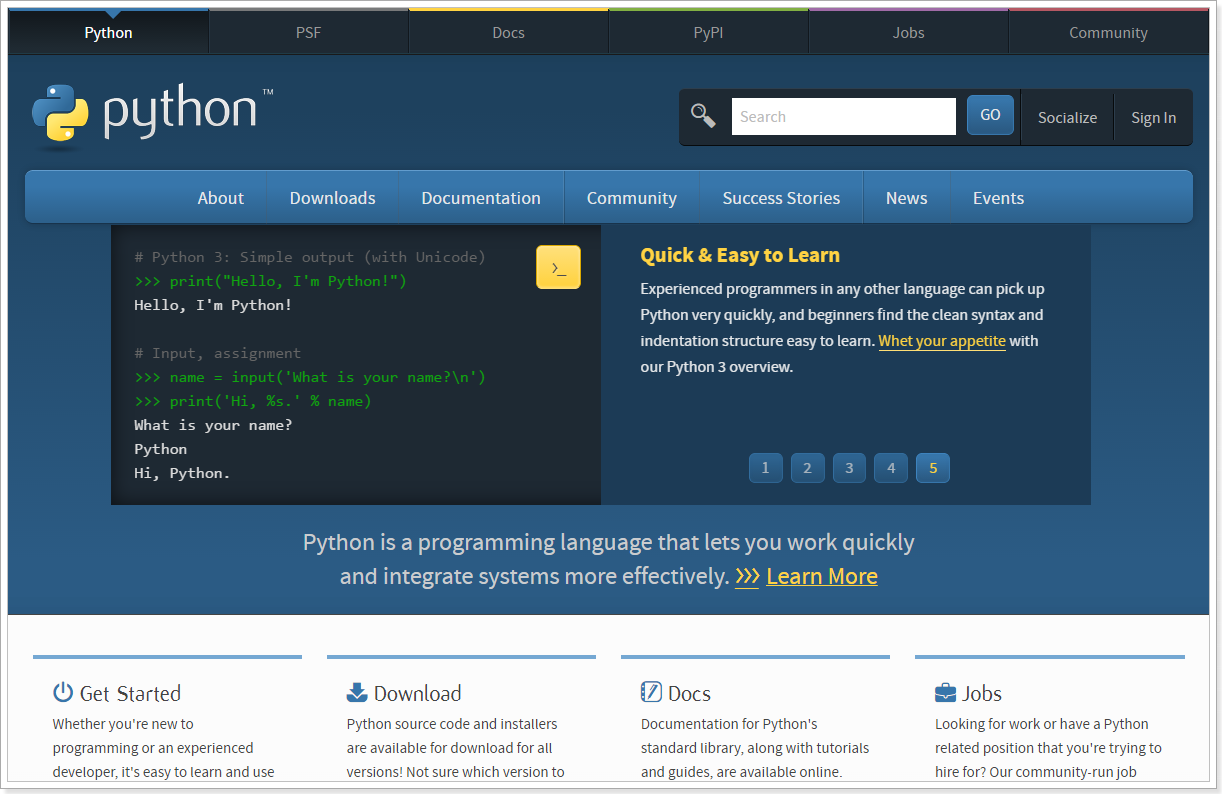
\includegraphics{Python-Download-001.png}
\end{quote}
\begin{itemize}
\item {} 
\href{https://www.python.org/downloads/}{Python Download} :進入下載頁面後,選擇『Download Python 3.x.x』下載Python3的版本

\end{itemize}
\begin{quote}

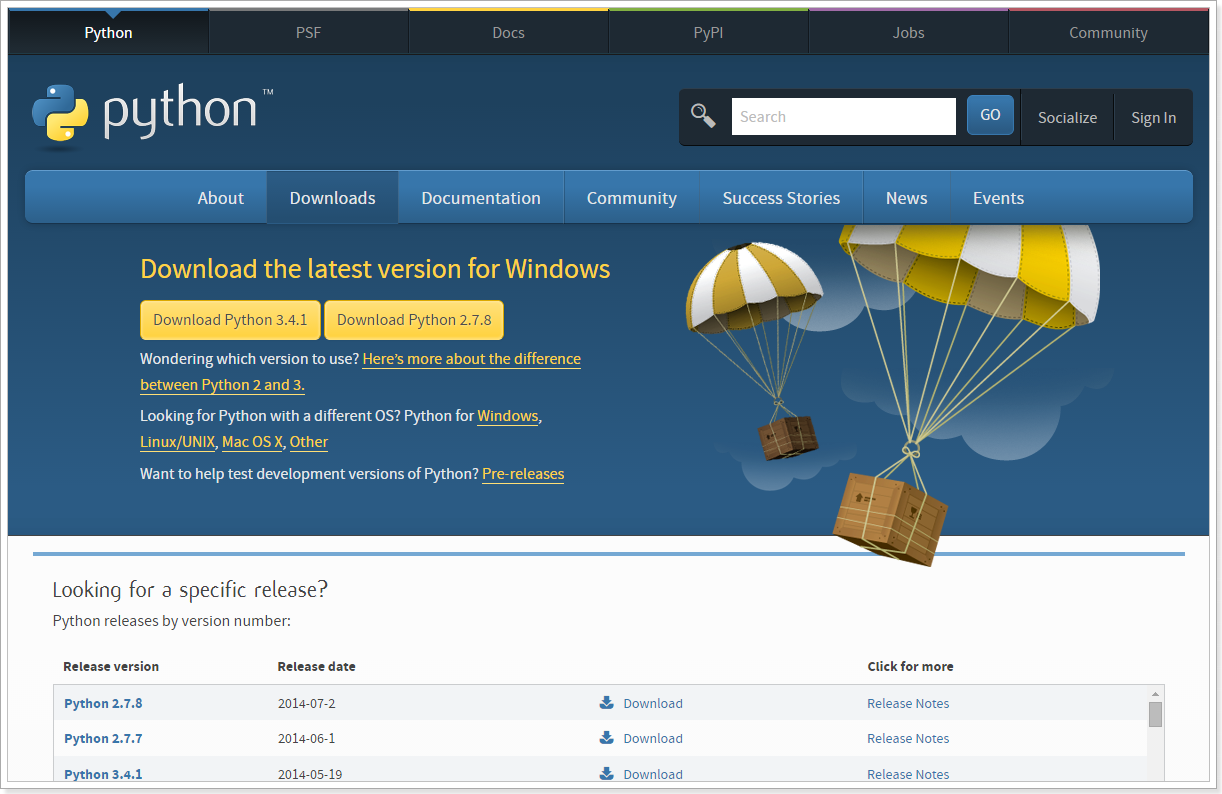
\includegraphics{Python-Download-002.png}
\end{quote}


\section{安裝 Python}
\label{_doc/sphinx-doc-win/index:id3}\begin{itemize}
\item {} 
執行Python安裝程式『python-3.4.1.msi』,使用預設值『Install for all users』

\end{itemize}
\begin{quote}

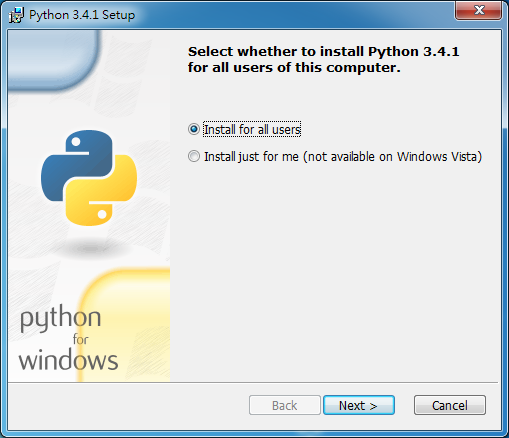
\includegraphics{Python-Install-001.png}
\end{quote}
\begin{itemize}
\item {} 
選擇安裝目錄,使用預設值『C:\textbackslash{}Python34\textbackslash{}』

\end{itemize}
\begin{quote}

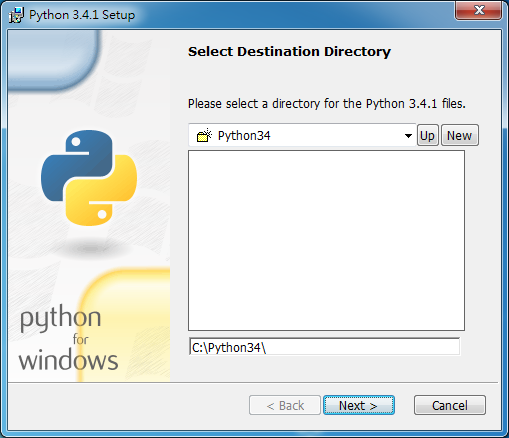
\includegraphics{Python-Install-002.png}
\end{quote}
\begin{itemize}
\item {} 
客製化安裝,這地方移到最後一個項目『Add python.exe to Path』,這預設是沒有選的,因為是第一次安裝,所以就把這個選項一起安裝,主要是將「C:\textbackslash{}Python34\textbackslash{};C:\textbackslash{}Python34\textbackslash{}Scripts;」這一串文字自動加入到環境變數的Path中,如果沒有選取安裝,需自行手動加入。

\end{itemize}
\begin{quote}

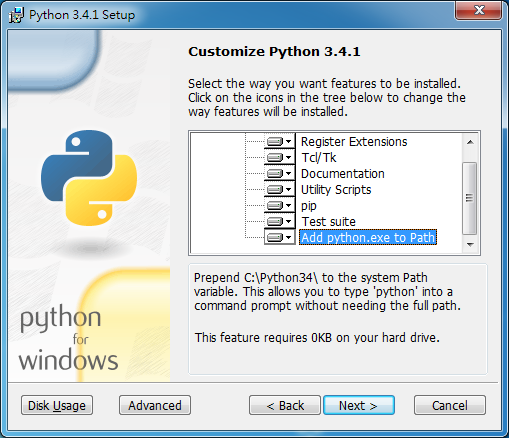
\includegraphics{Python-Install-003.png}
\end{quote}
\begin{itemize}
\item {} 
軟體安裝進度

\end{itemize}
\begin{quote}

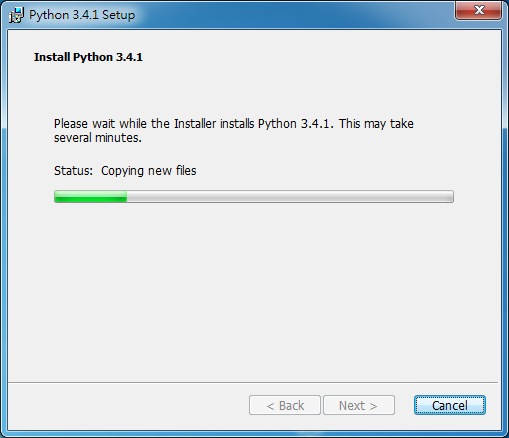
\includegraphics{Python-Install-004.png}
\end{quote}
\begin{itemize}
\item {} 
安裝完成

\end{itemize}
\begin{quote}

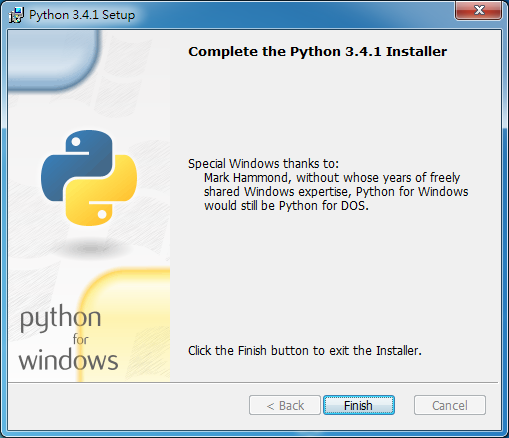
\includegraphics{Python-Install-005.png}
\end{quote}
\begin{itemize}
\item {} 
執行命令提示字元「開始-\textgreater{}所有程式-\textgreater{}附屬應用程式-\textgreater{}命令提示字元」,然後直接輸入『python』,就會看到如下的畫面,如果沒有請先確認系統環境變數的path是否有設定python的資料夾路徑「C:\textbackslash{}Python34\textbackslash{};C:\textbackslash{}Python34\textbackslash{}Scripts;」

\end{itemize}
\begin{quote}

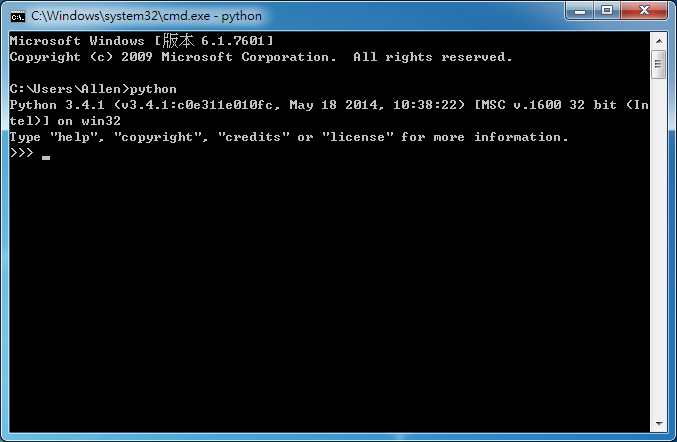
\includegraphics{Python-Install-006.png}
\end{quote}


\section{安裝easy\_install}
\label{_doc/sphinx-doc-win/index:easy-install}\begin{itemize}
\item {} 
下載 \href{https://bitbucket.org/pypa/setuptools/raw/bootstrap/ez\_setup.py}{ez\_setup.py} , 如下圖所下載的「ez\_setup.py」存放在「C:\textbackslash{}Users\textbackslash{}Allen\textbackslash{}」下並使用命令提示字元執行『python ez\_setup.py』

\end{itemize}
\begin{quote}

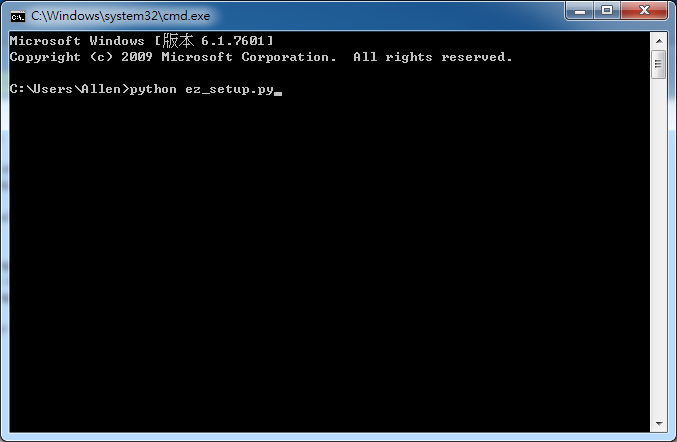
\includegraphics{Python-ezSetup-001.png}
\end{quote}
\begin{itemize}
\item {} 
下圖為安裝完會的畫面

\end{itemize}
\begin{quote}

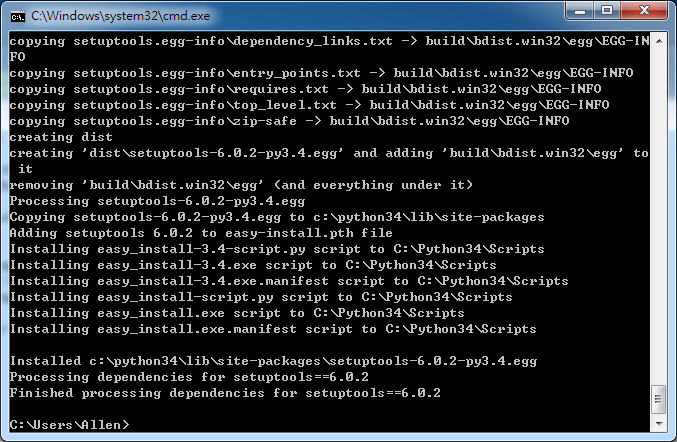
\includegraphics{Python-ezSetup-002.png}
\end{quote}


\section{安裝Sphinx}
\label{_doc/sphinx-doc-win/index:sphinx}\begin{itemize}
\item {} 
安裝好『easy\_install』,接著輸入『easy\_install sphinx』,安裝的時後需要一點時間

\end{itemize}
\begin{quote}

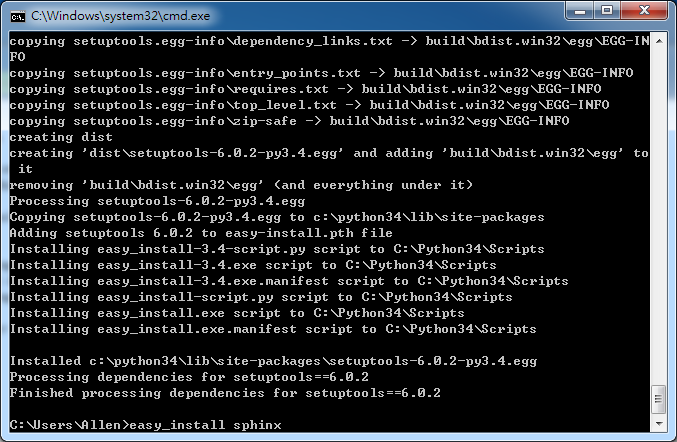
\includegraphics{Python-Sphinx-001.png}
\end{quote}
\begin{itemize}
\item {} 
下圖為安裝完成的畫面

\end{itemize}
\begin{quote}

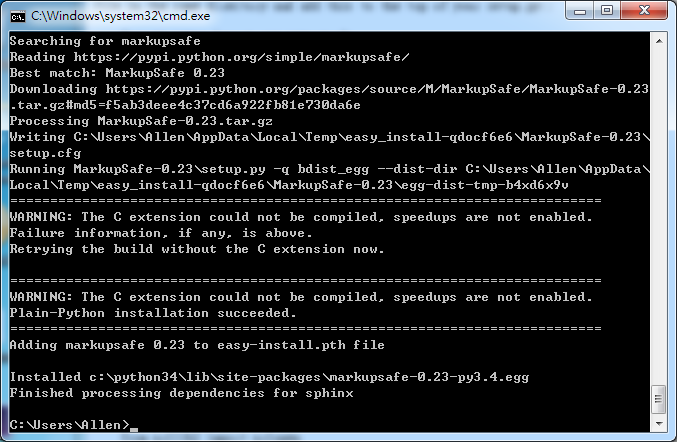
\includegraphics{Python-Sphinx-002.png}
\end{quote}
\begin{itemize}
\item {} 
安裝完成後,請輸入『sphinx-build』測試是否可以正常執行,如下圖

\end{itemize}
\begin{quote}

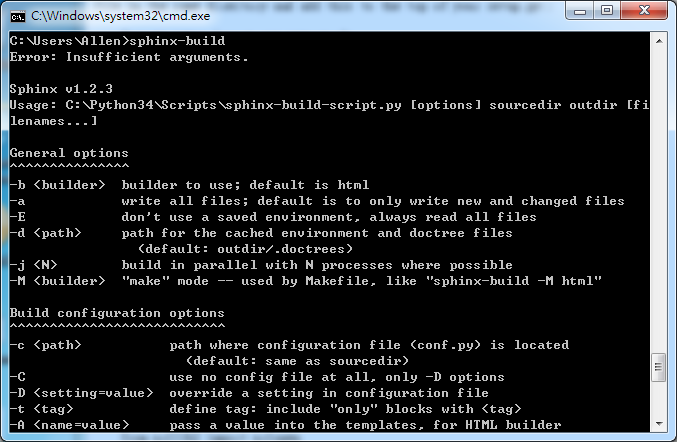
\includegraphics{Python-Sphinx-003.png}
\end{quote}


\section{參考網站連結}
\label{_doc/sphinx-doc-win/index:id4}\begin{itemize}
\item {} 
\href{http://sphinx-doc.org/install.html}{Sphinx-Doc Install}

\end{itemize}


\chapter{GIT、Gitolite3、Gitweb安裝}
\label{_doc/git/index::doc}\label{_doc/git/index:gitgitolite3gitweb}
在多人開發的過程中,為了便於整合不同使用者所建立的內容,在版本管控的多種系統中,如: \href{http://www.nongnu.org/cvs/}{CVS} 、 \href{http://subversion.apache.org/}{Subversion} 、 \href{http://git-scm.com/}{Git} 幾個主要的系統中選用Git當作開發的版本管控系統,主要為了之後可能會轉移到github上,再加上git的一些特性,如可快速的建立分支,不需中央伺服器即可在本地的檔案庫中做管理等…。

另外搭配 \href{http://gitolite.com}{Gitolite} 來管理使用者及檔案庫(Repository),讓管理者便於設定檔案庫的存取權限,Gitolite綁定一個系統帳號,而其他的使用者都是透過ssh key建立,只要把key的名稱設定權限後,即可設定key及檔案庫的讀寫、執行或只能讀取等,並透過gitweb讓使用者用瀏覽器就可以觀看檔案庫的內容、記錄、版本差異、下載等功能。


\section{GIT安裝}
\label{_doc/git/index:id1}
\textbf{安裝GIT}
\begin{quote}

\begin{Verbatim}[commandchars=\\\{\}]
sudo apt\PYGZhy{}get install git\PYGZhy{}core
\end{Verbatim}
\end{quote}

\textbf{新增使用者git}
\begin{quote}

\begin{Verbatim}[commandchars=\\\{\}]
sudo useradd \PYGZhy{}m git
sudo passwd git
\end{Verbatim}
\end{quote}

\textbf{設置使用者的git全域參數}
\begin{quote}

\begin{Verbatim}[commandchars=\\\{\}]
sudo su \PYGZhy{}l git
git config \PYGZhy{}\PYGZhy{}global user.name \PYGZdq{}username\PYGZdq{}
git config \PYGZhy{}\PYGZhy{}global user.email \PYGZdq{}email\PYGZdq{}
\end{Verbatim}
\end{quote}


\section{Gitolite3安裝}
\label{_doc/git/index:gitolite3}\begin{quote}

在安裝過程式會出現Configuring gitolite3的畫面,要輸入Administrator's SSH key,如果尚未產生好ssh key的話可以跳過,之後再設定使用sudo dpkg-reconfigure gitolite3就可以重新設定
\end{quote}

\textbf{安裝gitolite3}
\begin{quote}

\begin{Verbatim}[commandchars=\\\{\}]
sudo apt\PYGZhy{}get install gitolite3
\end{Verbatim}
\end{quote}

\textbf{執行畫面}
\begin{quote}

\begin{Verbatim}[commandchars=\\\{\}]
allen@uServer:/home/git⟫ sudo apt\PYGZhy{}get install gitolite3
[sudo] password for allen:
Reading package lists... Done
Building dependency tree
Reading state information... Done
Suggested packages:
  git\PYGZhy{}daemon\PYGZhy{}run gitweb
The following NEW packages will be installed:
  gitolite3
0 upgraded, 1 newly installed, 0 to remove and 0 not upgraded.
Need to get 85.3 kB of archives.
After this operation, 352 kB of additional disk space will be used.
Get:1 http://opensource.nchc.org.tw/ubuntu/ trusty/universe gitolite3 all 3.5.3.1\PYGZhy{}2 [85.3 kB]
Fetched 85.3 kB in 5s (16.6 kB/s)
Preconfiguring packages ...
Selecting previously unselected package gitolite3.
(Reading database ... 121302 files and directories currently installed.)
Preparing to unpack .../gitolite3\PYGZus{}3.5.3.1\PYGZhy{}2\PYGZus{}all.deb ...
Unpacking gitolite3 (3.5.3.1\PYGZhy{}2) ...
Processing triggers for man\PYGZhy{}db (2.6.7.1\PYGZhy{}1) ...
Setting up gitolite3 (3.5.3.1\PYGZhy{}2) ...
No adminkey given \PYGZhy{} not setting up gitolite. Do a dpkg\PYGZhy{}reconfigure to setup.
allen@uServer:/home/git⟫
\end{Verbatim}

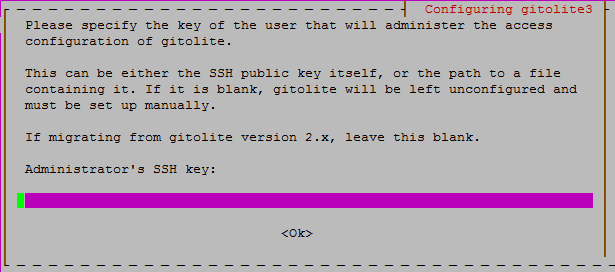
\includegraphics{gitolite3-configureing.png}
\end{quote}

\textbf{產生git ssh key}
\begin{quote}

用ssh-keygen指令產生,一般用 \emph{ssh-keygen -t rsa} 即可產生公鑰、私鑰,預設會建立在家目前中的「.ssh」資料夾中,在建立的過程式可以自行修改公、私鑰的位置及檔名,公鑰預設檔案名稱為「\textasciitilde{}/.ssh/id\_rsa」,,私龠預設檔案名為「\textasciitilde{}/.ssh/id\_rsa.pub」,在產生公、私鑰的過程會要輸入passphrase,預設值是空的,如果要使用密碼請在這裡輸入後再按Enter,這樣之後連線時就會要輸入密碼後才可以登入。如下圖..

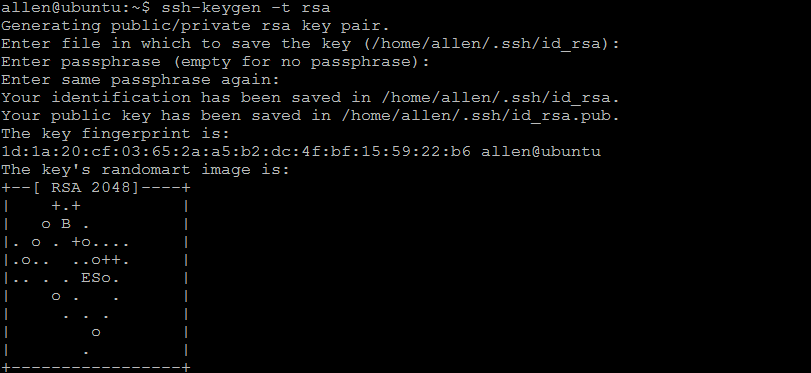
\includegraphics{ssh-keygen.png}

以上說的內容可以直接用指令執行後即可產生公、私鑰,「-P」加入密碼(passphrase),「-f」檔案產生的位置與名稱,如下
\end{quote}

\textbf{ssh-keygen指令}
\begin{quote}

\begin{Verbatim}[commandchars=\\\{\}]
ssh\PYGZhy{}keygen \PYGZhy{}t rsa \PYGZhy{}P \PYGZsq{}admin@gitolite\PYGZsq{} \PYGZhy{}f \PYGZti{}/.ssh/admin
\end{Verbatim}

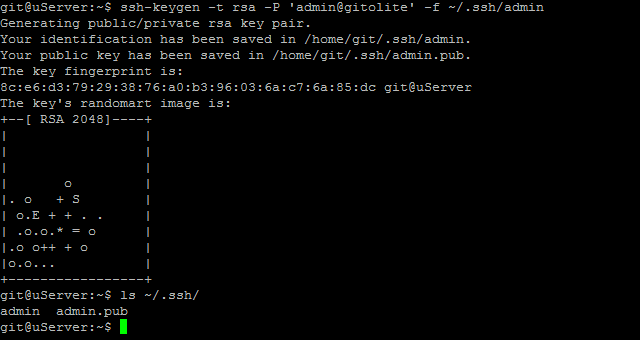
\includegraphics{ssh-keygen2.png}
\end{quote}

\textbf{設定配置gitolite3}
\begin{quote}

執行下方的設定配置指令後會出現設定畫面,首先出現的是設定gitolite3的系統管理者,在這邊我們預設定的系統管理者為「git」

\begin{Verbatim}[commandchars=\\\{\}]
sudo dpkg\PYGZhy{}reconfigure gitolite3
\end{Verbatim}

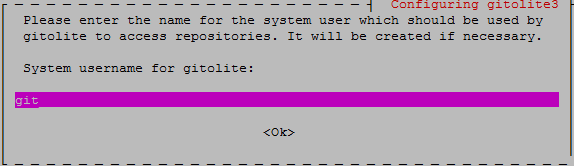
\includegraphics{gitolite3-username.png}

設定「Repository」資料夾路徑,把Repository設在使用者git的家目錄下

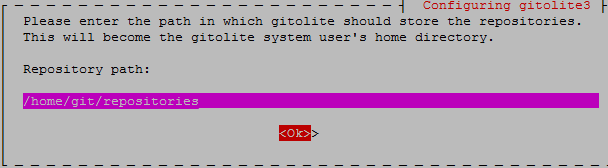
\includegraphics{gitolite3-repository-path.png}

接著又回到一開始安裝時要設定的管理者ssh key,這裡用上面所設定admin.pub,要輸入完整的路徑

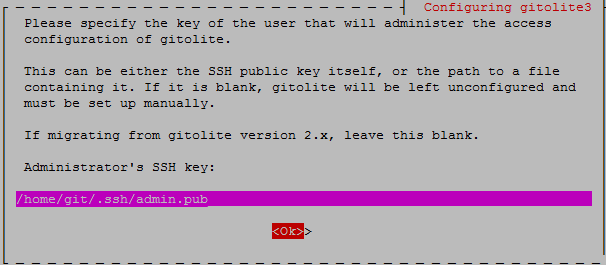
\includegraphics{gitolite3-admin-sshkey.png}

確認後就會看到下面的畫面,在repositories中將會自動產生兩個repo「gitolite-admin.git及testing.git」及一個projects.list,如下圖

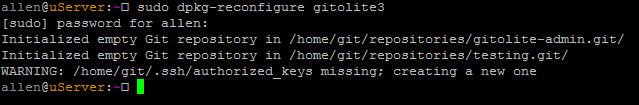
\includegraphics{gitolite3-cmd.png}

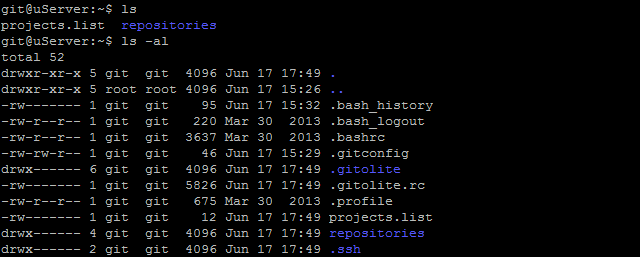
\includegraphics{gitolite3-list.png}
\end{quote}

\textbf{設定gitolite-admin}
\begin{quote}

gitolite-admin主要是用於設定及管理repo與使用者,此外可以設定每個repo的存取權限,gitolite-admin預設只供管理者存取,所以要用設定gitolit3時所設定的administrator's ssh key來存取設定。

目前使用git使用者,也在此使用者建立ssh key,當做gitolite3的管理者,所以先登入git,並在家目錄中clone gitolite-admin做設定

\begin{Verbatim}[commandchars=\\\{\}]
git clone git@localhost:gitolite\PYGZhy{}admin.git
\end{Verbatim}

在git的家目錄把gitolite-admin取出後,進到gitolite-admin資料夾,將會有兩個檔案,分別為「conf/gitolite.conf」與「keydir/admin.pub」

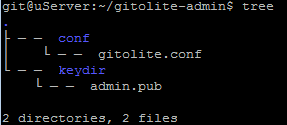
\includegraphics{gitolite3-admin-tree.png}

「conf/gitolite.conf」預設的內容如下,在gitolite-admin目前設定只供admin做讀寫及更新,其他使用者無法

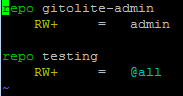
\includegraphics{gitolite3-admin-config.png}

「keydir/admin.pub」keydir資料夾是放使用者ssh公鑰的地方,此資料夾中的admin.pub就是在設定gitolite時所輸入的administrator's ssh key。
\end{quote}

\textbf{Linux 新增使用者到gitolite3}
\begin{quote}

先在自已家目錄中執行ssh-keygen -t rsa 產生公、私鑰,預設會存在\textasciitilde{}/.ssh/下,將公鑰id\_rsa.pub更換名稱,例如目前帳號使用allen,則把id\_rsa.pub改成allen.pub,並且把 allen.pub放到gitolite-admin/keydir資料夾下,使用者的公鑰部分可以放到「/tmp」下,這樣切換到時用者時就不需再另外更改檔案擁有者及權限。

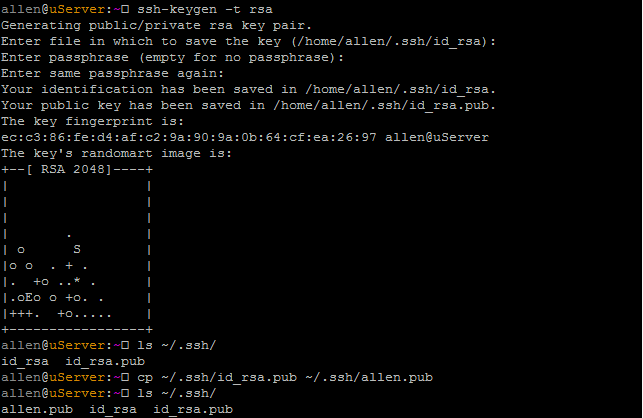
\includegraphics{gitolite3-adduser-1.png}

在使用者allen下就先cp一份公鑰到/tmp下,

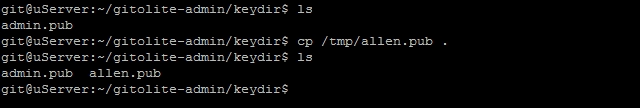
\includegraphics{gitolite3-adduser-2.png}

接下來就執行git指令,把使用者的公鑰放到gitolite-admin repo中,在過程中有出現「Enter passphrase for key...」這部分因為在建立admin公、私鑰時有輸入密碼,所以在這個時後就需要輸入之前的密碼以確定執行git push上傳更新。

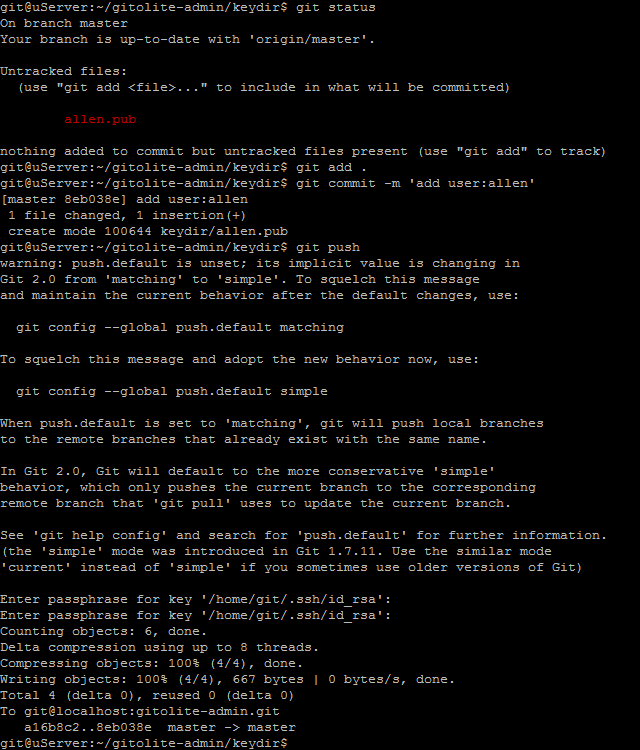
\includegraphics{gitolite3-adduser-3.png}
\end{quote}

\textbf{新增GIT Repo}
\begin{quote}

使用者新增好了之後,我將建立一個給allen專用的repo,加入了

\begin{Verbatim}[commandchars=\\\{\}]
repo allen
        RW+ = allen
\end{Verbatim}

這樣設定在gitweb預設不會將repo列出,如果要供大家讀取,則再加入一行即可

\begin{Verbatim}[commandchars=\\\{\}]
R     =  @all
\end{Verbatim}

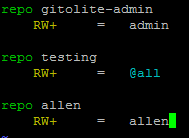
\includegraphics{gitolite3-addrepo-1.png}

接著做相同的動作,如下

\begin{Verbatim}[commandchars=\\\{\}]
git add .
git commit \PYGZhy{}m \PYGZsq{}add repo:allen\PYGZsq{}
git push
\end{Verbatim}

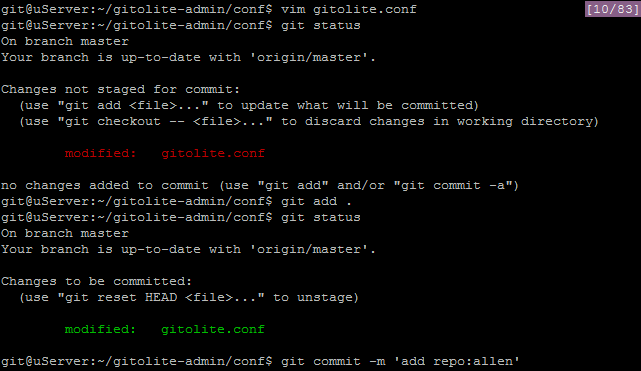
\includegraphics{gitolite3-addrepo-2.png}

當執行git指令,把設定檔更新後,回到「\textasciitilde{}/repositories」中,將會看到自已建立了一個repo「allen.git」

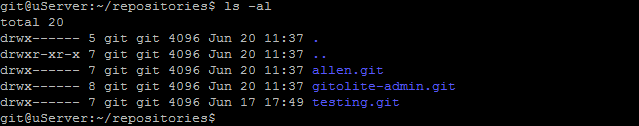
\includegraphics{gitolite3-addrepo-3.png}

用使用者allen 去clone allen.git,執行完後會如下圖,將會在執行的目錄中增加一個allen的git repo,預設裡面是空的,只有一個.git的設定檔資料夾

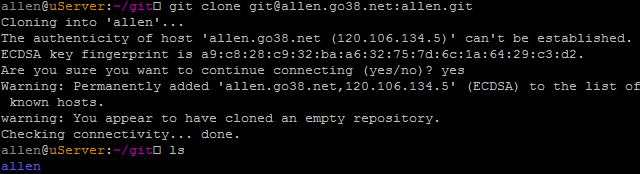
\includegraphics{gitolite3-addrepo-4.png}
\end{quote}

\textbf{repo初始內容}
\begin{quote}

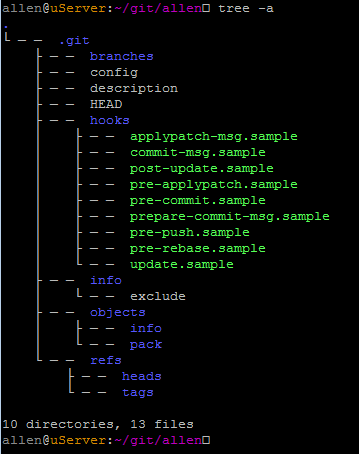
\includegraphics{gitolite3-addrepo-5.png}
\end{quote}


\section{安裝GitWeb}
\label{_doc/git/index:gitweb}
\textbf{安装apache2}
\begin{quote}

\begin{Verbatim}[commandchars=\\\{\}]
sudo apt\PYGZhy{}get install apache2
\end{Verbatim}
\end{quote}

\textbf{設定啟用cgi}
\begin{quote}

\begin{Verbatim}[commandchars=\\\{\}]
sudo vim /etc/apache2/sites\PYGZhy{}enabled/000\PYGZhy{}default.conf
把這行前方的\PYGZsh{}拿掉 「Include conf\PYGZhy{}available/serve\PYGZhy{}cgi\PYGZhy{}bin.conf」
sudo a2enmod cgi
sudo apache2 restart
\end{Verbatim}

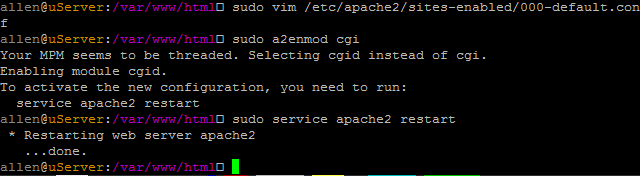
\includegraphics{gitolite3-cgi-1.png}
\end{quote}

\textbf{安裝gitweb}
\begin{quote}

\begin{Verbatim}[commandchars=\\\{\}]
sudo apt\PYGZhy{}get install gitweb
\end{Verbatim}
\end{quote}

\textbf{設定gitweb}
\begin{quote}

安裝完後資料放在預設目錄「/usr/share/gitweb/」下,而設定檔放在「/etc/gitweb.conf」,apache2的預設目錄「/var/www/html」,將gitweb會讀取到的相關css及圖檔資料夾static做連結到網站的根目錄

\begin{Verbatim}[commandchars=\\\{\}]
sudo ln \PYGZhy{}s /usr/share/gitweb/static /var/www/html
\end{Verbatim}

編輯gitweb.conf設定參數如下圖

\begin{Verbatim}[commandchars=\\\{\}]
sudo vim /etc/gitweb.conf
\end{Verbatim}

注意\$projectroot,\$projects\_list要改成自已所設定的路徑

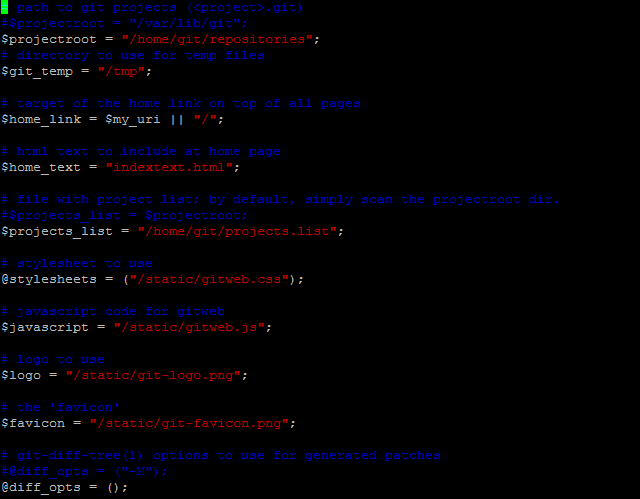
\includegraphics{gitolite3-gitweb-1.png}
\end{quote}
\begin{description}
\item[{\textbf{gitweb權限設定}}] \leavevmode
當設定好後啟動apache2,用瀏灠器進入 \href{http://localhost/cgi-bin/gitweb.cgi}{http://localhost/cgi-bin/gitweb.cgi} 會發現出現404,並沒有repo專案出現,在這裡需要做算讀取權限的設定

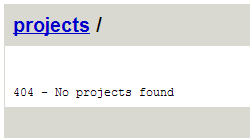
\includegraphics{gitolite3-gitweb-2.png}

將git加入群組www-data

\begin{Verbatim}[commandchars=\\\{\}]
sudo usermod \PYGZhy{}a \PYGZhy{}G git www\PYGZhy{}data
\end{Verbatim}

資料夾repositories設定為755
檔案projects.list設定為644
資料夾repositories中的repo,原本資料夾權限預設為700,群組的部分不能讀取,如果要開放的話,請將該xxx.git資料夾設定為755,如下方指令要開放testing.git,

\begin{Verbatim}[commandchars=\\\{\}]
chmod 755 \PYGZhy{}R testing.git
\end{Verbatim}

當設定以上的權限後重新啟動apache2即可看到所開放的repo,但如果使用者有做git push後會發現,網頁上該被push過的repo又不見了,但再執行一次chmod 755 -R testing.git後網頁上又出現了,發現在push後有些資料夾的權限會變成預設的700,所以要再做下面的修改,將設定repo預設的建立權限為750,這樣使用者在做push更新時,相關檔案建立時www-data群組就可以做存取的動作,修改如下

在使用者git家目錄下

\begin{Verbatim}[commandchars=\\\{\}]
vim \PYGZti{}/.gitolite.rc
\end{Verbatim}

將UMASK的預設值0077改成0027後,存儲並重新啟動apache2,再重新push一次後就會發相部分相關檔案在push後所建立的權限為750,並且gitweb網頁也可以正常的觀看。

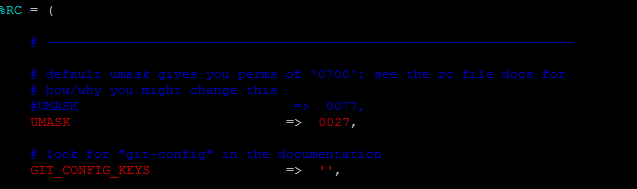
\includegraphics{gitolite3-gitweb-3.png}

\end{description}


\section{參考網站連結}
\label{_doc/git/index:id2}\begin{itemize}
\item {} 
Git 版本控制系統 \href{http://ihower.tw/git/index.html}{http://ihower.tw/git/index.html}

\item {} 
30天精通Git版本控管 \href{http://ithelp.ithome.com.tw/ironman6/player/doggy/dev/1}{http://ithelp.ithome.com.tw/ironman6/player/doggy/dev/1}

\item {} 
Git Community Book 中文版 \href{http://gitbook.liuhui998.com/index.html}{http://gitbook.liuhui998.com/index.html}

\item {} 
Pro Git Book \href{http://git-scm.com/book/zh-tw}{http://git-scm.com/book/zh-tw}

\end{itemize}


\chapter{Git Hooks}
\label{_doc/git/git_hooks::doc}\label{_doc/git/git_hooks:git-hooks}
test

test2

test3

test4

test5

test6

test7


\section{相關連結}
\label{_doc/git/git_hooks:id1}
\href{http://git-scm.com/book/zh-tw/Git-客製化-Git-Hooks}{Git 客製化 - Git Hooks}
\href{https://github.com/xPaw/GitHub-WebHook}{GitHub-WebHook}


\chapter{共同寫作操作流程}
\label{_doc/writing/index::doc}\label{_doc/writing/index:id1}

\section{相關軟體安裝}
\label{_doc/writing/index:id2}\begin{enumerate}
\item {} 
\href{https://code.google.com/p/tortoisegit/}{TortoiseGit} (安裝教學)

\item {} 
\href{http://www.git-scm.com/download/win}{Git} (安裝教學)

\end{enumerate}


\section{建立使用者帳號(SSH-KEY)}
\label{_doc/writing/index:ssh-key}
在安裝好TortoiseGit與Git後,使用此軟體建立ssh公鑰(Public Key)與私鑰(Private Key),安裝的兩個軟體都可以建立ssh-key,使用安裝TortoiseGit附帶一起安裝的 \href{http://www.chiark.greenend.org.uk/~sgtatham/putty/download.html}{Puttygen} 建立,此方式是有圖形介面(GUI),較容易看到所產生的內容,操作方式請參照 {\hyperref[_doc/writing/index:ssh-key-puttygen]{\emph{Puttygen建立ssh-key}}},如果要使用Git Bash建立ssh-key請參照 {\hyperref[_doc/writing/index:ssh-key-gitbash]{\emph{Git Bash建立ssh-key}}},此方式是屬於文字介面,操作方式如Windows的『命令題示字元模式』與Linux的『console模式』,但操作的指令比較像Linux的console模式。


\subsection{Puttygen建立ssh-key}
\label{_doc/writing/index:puttygenssh-key}\label{_doc/writing/index:ssh-key-puttygen}\begin{itemize}
\item {} 
啟動Puttygen,打開『開始程式集』,找到 \textbf{TortoiseGit} 點選打開後就會看到如下圖的內容,點選執行『Puttygen』

\end{itemize}
\begin{quote}

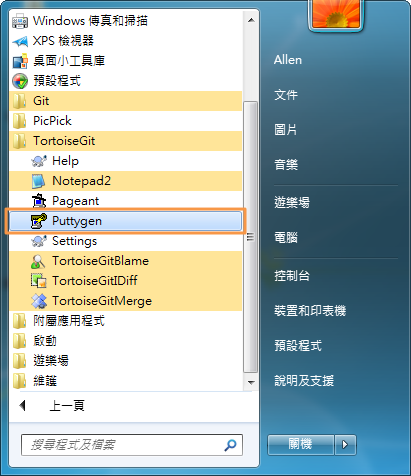
\includegraphics{puttygen-001.png}
\end{quote}
\begin{itemize}
\item {} 
啟動Puttygen後的畫面如下

\end{itemize}
\begin{quote}

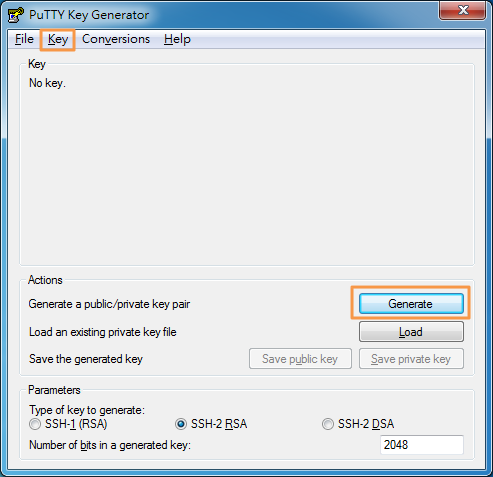
\includegraphics{puttygen-002.png}
\end{quote}
\begin{itemize}
\item {} 
點選畫面中的『Generate』,或者是上方選單的『Key-\textgreater{}Generate key pair』,點選後會看到畫面上多了一串字『Please generate some randmness by moving the mouse over the blank area.』,簡單來說就是『請在key的空白區塊移動滑鼠以產生ssh-key』及一個Process Bar以顯示ssh-key產生的進度。

\end{itemize}
\begin{quote}

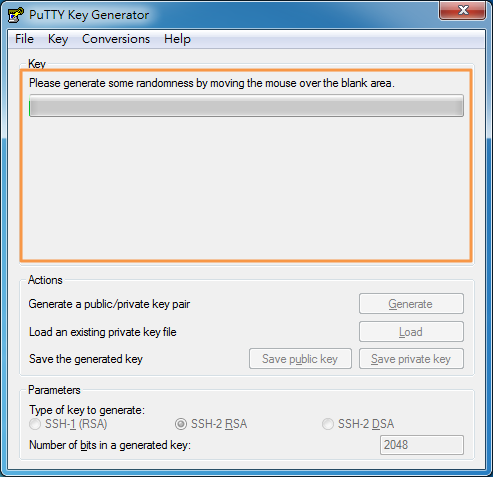
\includegraphics{puttygen-003.png}
\end{quote}
\begin{itemize}
\item {} 
不斷的在key的空白區塊移動滑鼠時,Process Bar的目前進度就會一直增加

\end{itemize}
\begin{quote}

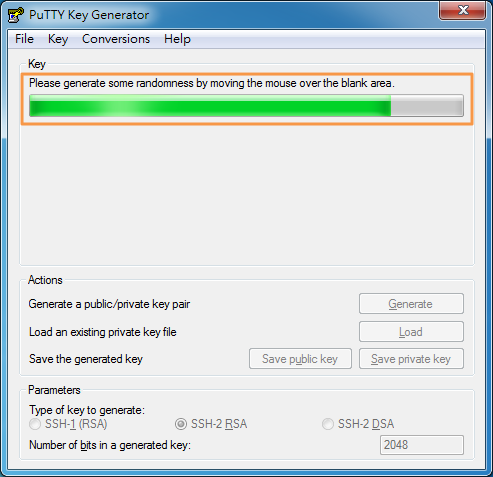
\includegraphics{puttygen-004.png}
\end{quote}
\begin{itemize}
\item {} 
當Process Bar跑完全都變綠色時,代表已完成產生ssh-key,這時key的空白區塊就會改變成顯示所產生的ssh-key

\end{itemize}
\begin{quote}

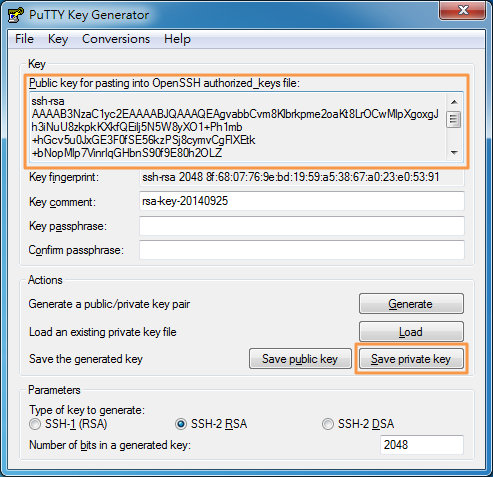
\includegraphics{puttygen-005.png}
\end{quote}
\begin{itemize}
\item {} 
這時可用下方的『Save private key』按鈕來儲存私鑰,點選按鈕後會跳出存儲視窗,先選擇要存放的資料夾,接著在檔案名稱的地方輸入檔名,副檔名為『ppk』,最後點選存檔即可。

公鑰正常來說也是點選『Save public key』然後一樣的方式就可以完成,但發現直接存檔,把此公鑰放在伺服器上面時會無法正常使用,最後發現因為在每64個字母後面就加一個空白,因為此空白造成上傳到伺服器時無法正常的運作,只要用文字編輯器打開,將每64個字母後方的空白刪除後存檔即可,另外一個方式就是將『Public key for pasting into OpenSSH authorized\_keys file:』下方區塊的內容全選複製,然後打開文字編輯器,貼上所選取的public key,再儲存檔案就可以了,公鑰的副檔名為『pub』。

建議:公鑰部分,直接複製貼上畫面中的Public key,避免在刪除空白時不小時刪錯,造成無法使用。

\end{itemize}
\begin{quote}

\textbf{點選『Save public key』所儲存的內容如下}

\begin{Verbatim}[commandchars=\\\{\}]
\PYGZhy{}\PYGZhy{}\PYGZhy{}\PYGZhy{} BEGIN SSH2 PUBLIC KEY \PYGZhy{}\PYGZhy{}\PYGZhy{}\PYGZhy{}
Comment: \PYGZdq{}rsa\PYGZhy{}key\PYGZhy{}20140925\PYGZdq{}
AAAAB3NzaC1yc2EAAAABJQAAAQEAieoX4nQSi9b0wm5phNZA7wimvtBLiK37IUcG
YzGX0FukwmPDF6hZlqIvxwPHn5QvluI4EIFdTH1ybWAhlK8awmQuoSKkaFwRxM8q
x2DXyHdHGTwbFjNSnh/mRD9dNrROkXfqqkb7SyT5wGfi5dDRpquo9y8Mv8kkXkUo
x0olI7bT377FBT1Yl9VAFIF9PpNeBYpwI+lKR5aB6q7ABx5ynWo6YFDVPN03czBl
lslrSo7/Y3r1vB8r0zxSyTMj8OXo4ZirzefwOc1ge8fpfs0XiGgOT6FrTerXzxWE
zF7Scl15SdLsz122G4znCpf3AIQ795Zcwg5/Qpm9KFJ/6gUl/Q==
\PYGZhy{}\PYGZhy{}\PYGZhy{}\PYGZhy{} END SSH2 PUBLIC KEY \PYGZhy{}\PYGZhy{}\PYGZhy{}\PYGZhy{}
\end{Verbatim}

\textbf{將儲存的內容刪除每64個字母後方的空白}

\begin{Verbatim}[commandchars=\\\{\}]
\PYGZhy{}\PYGZhy{}\PYGZhy{}\PYGZhy{} BEGIN SSH2 PUBLIC KEY \PYGZhy{}\PYGZhy{}\PYGZhy{}\PYGZhy{}
Comment: \PYGZdq{}rsa\PYGZhy{}key\PYGZhy{}20140925\PYGZdq{}
AAAAB3NzaC1yc2EAAAABJQAAAQEAieoX4nQSi9b0wm5phNZA7wimvtBLiK37IUcGYzGX0FukwmPDF6hZlqIvxwPHn5QvluI4EIFdTH1ybWAhlK8awmQuoSKkaFwRxM8qx2DXyHdHGTwbFjNSnh/mRD9dNrROkXfqqkb7SyT5wGfi5dDRpquo9y8Mv8kkXkUox0olI7bT377FBT1Yl9VAFIF9PpNeBYpwI+lKR5aB6q7ABx5ynWo6YFDVPN03czBllslrSo7/Y3r1vB8r0zxSyTMj8OXo4ZirzefwOc1ge8fpfs0XiGgOT6FrTerXzxWEzF7Scl15SdLsz122G4znCpf3AIQ795Zcwg5/Qpm9KFJ/6gUl/Q==
\PYGZhy{}\PYGZhy{}\PYGZhy{}\PYGZhy{} END SSH2 PUBLIC KEY \PYGZhy{}\PYGZhy{}\PYGZhy{}\PYGZhy{}
\end{Verbatim}
\end{quote}
\begin{itemize}
\item {} 
當執行完畢後,將會在所存放的資料夾內容看到公鑰(user2.pub)與私鑰(user2.ppk)

\end{itemize}
\begin{quote}

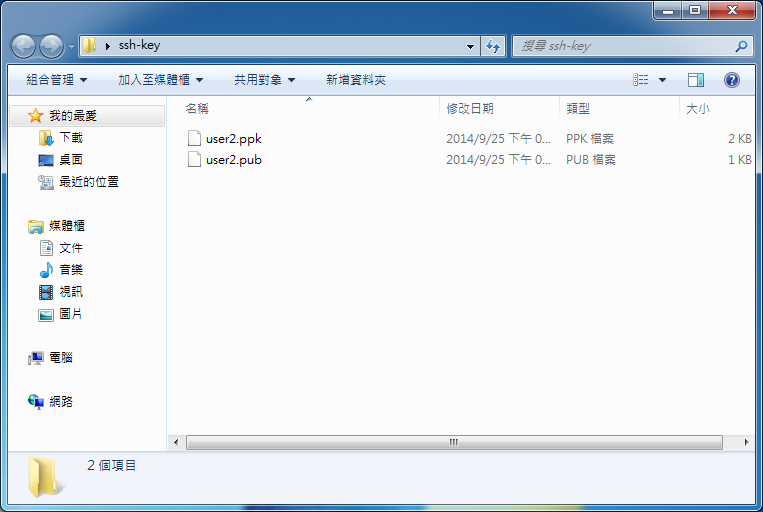
\includegraphics{puttygen-006.png}
\end{quote}


\subsection{Git Bash建立ssh-key}
\label{_doc/writing/index:ssh-key-gitbash}\label{_doc/writing/index:git-bashssh-key}\begin{itemize}
\item {} 
啟動Git Bash,打開『開始程式集』,找到 Git 點選打開後就會看到如下圖的內容,點選執行『Git Bash』

\end{itemize}
\begin{quote}

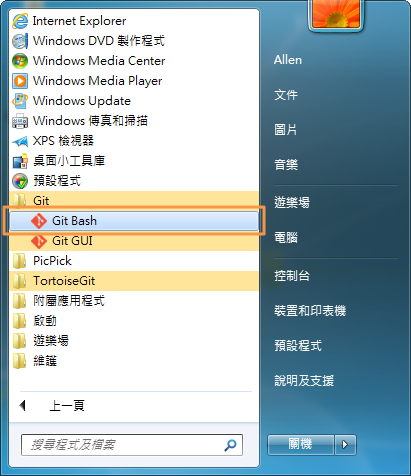
\includegraphics{gitBash-001.png}
\end{quote}
\begin{itemize}
\item {} 
建立ssh-key的指令

\end{itemize}
\begin{quote}

\begin{Verbatim}[commandchars=\\\{\}]
ssh\PYGZhy{}keygen \PYGZhy{}t rsa \PYGZhy{}C \PYGZdq{}user2@host\PYGZdq{}
\end{Verbatim}

進入畫面後,可以先用pwd確認目前的資料夾路徑,然後進入到想要存放ssh公鑰(Public Key)與私鑰(Private Key)的資料夾,然後執行『ssh-keygen -t rsa』即可,『-C ``\href{mailto:user2@host}{user2@host}``』這是加入註解說明文字,有加這個參數,會將雙引號中的文字加在所產生ssh-key的最後方,在建立過程會出現『Enter passphrase』這部分如果是空白沒有輸入密碼,在使用git操作時將不會要求輸入密碼,反之,在這些輸入密碼後,在操作git也會出現要輸入密碼訊息,輸入正確的密碼後才會執行git指令。

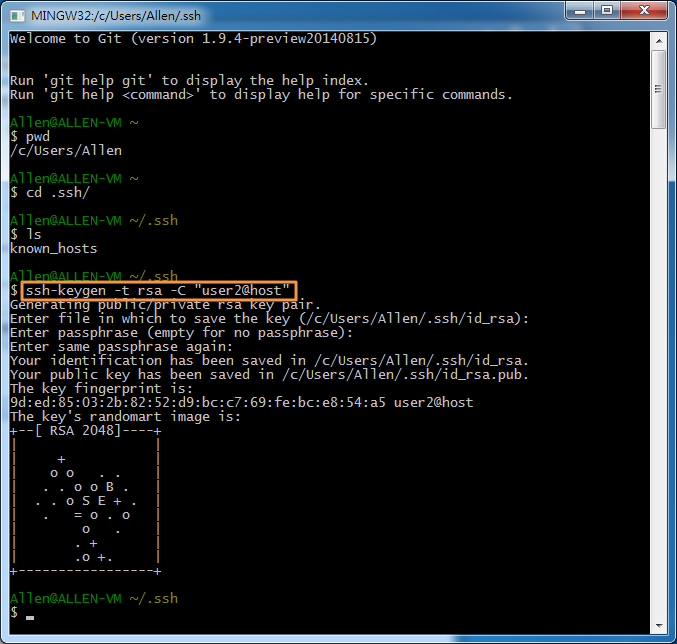
\includegraphics{gitBash-002.png}
\end{quote}
\begin{itemize}
\item {} 
執行完後,可以輸入『ls -al』列出目前資料夾產生了什麼檔案,基本上會出現公鑰(id\_rsa.pub)與私鑰(id\_rsa)這兩個檔案,接著將公鑰(id\_rsa.pub)複製成另一個檔案,例如目前的使用者名稱為user2,所以執行『cp id\_rsa.pub user2.pub』,再次執行『ls -al』檢查資料夾中是否有新增一個『user2.pub』檔案。

\end{itemize}
\begin{quote}

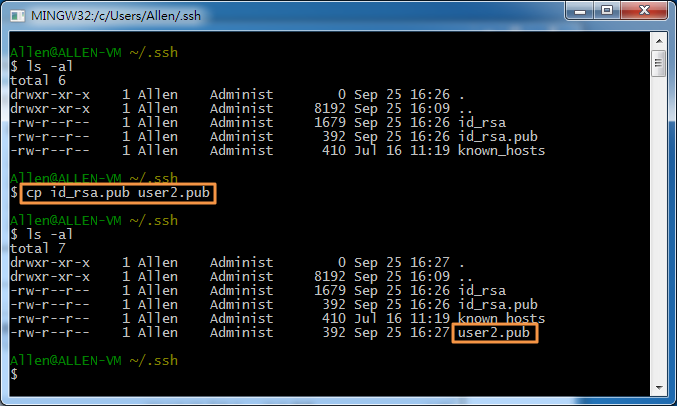
\includegraphics{gitBash-003.png}
\end{quote}
\begin{itemize}
\item {} 
ssh-keygen指令說明,可以執行『ssh-keygen -h』將會列出如下圖的內容

\end{itemize}
\begin{quote}

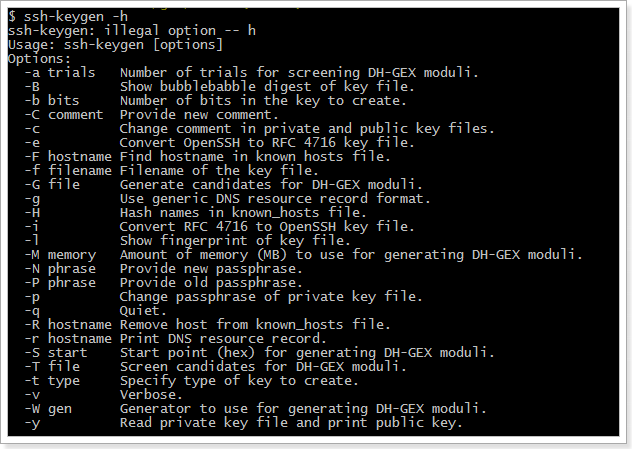
\includegraphics{ssh-keygen-help.png}
\end{quote}


\subsubsection{轉換Git Bash產生的私鑰格式}
\label{_doc/writing/index:git-bash}\begin{itemize}
\item {} 
當使用 {\hyperref[_doc/writing/index:ssh-key-gitbash]{\emph{Git Bash建立ssh-key}}} 的方式建立ssh公鑰(Public Key)與私鑰(Private Key)後,在之後使用Pgageant做連線時會出現下面的視窗, 顯示所選擇的key不能載入,因為格式為OpenSSH而所使用的工具是Putty系列的工具,所以需要做一下式格的轉換

\end{itemize}
\begin{quote}

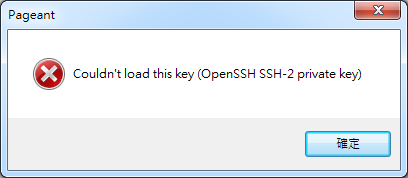
\includegraphics{openssh-putty-001.png}
\end{quote}
\begin{itemize}
\item {} 
注意一下在Git Bash產生ssh-key後,的內容,會有兩個檔案,在私鑰的部分是沒有副檔名ppk的,

\end{itemize}
\begin{quote}

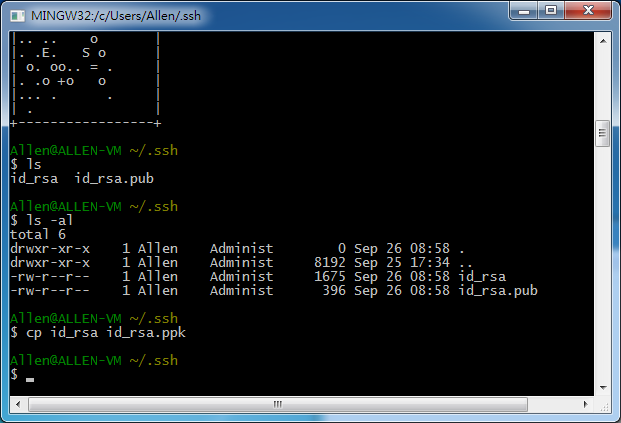
\includegraphics{openssh-putty-002.png}

\textbf{Git Bash產生的私鑰格式}

\begin{Verbatim}[commandchars=\\\{\}]
\PYGZhy{}\PYGZhy{}\PYGZhy{}\PYGZhy{}\PYGZhy{}BEGIN RSA PRIVATE KEY\PYGZhy{}\PYGZhy{}\PYGZhy{}\PYGZhy{}\PYGZhy{}
MIIEowIBAAKCAQEA21wVMmtJSprBBhBifFDyIvTMdFd3oGQw4XegQunAR0N/MdGd
aQSJdOJzljkd8lpOXnpkdBjfpnvxQOO9Ad0QbpfLu1/hOb/74S8MlIvc3tHPmefd
DDDAGokEd8vevJGyXceLv6yIoZxgNP9npDAE1k+DiHAVUtk3IBMxaP6bUy36RZbx
CakSemFqGtO2L51/9YI4j3LmGbbnHh8K4YLD9dHfbey7CN3KgvPKkptW/49LrbWZ
QhWl6mXGRWfSIwWEML6B+EsUFqwhVte9TFTtxINJa3cvHwbxmsgmVP51M0MiWpUf
iK7LM4BdW7dpy5KW+FzGj5UwVxpoku2HRRA14wIDAQABAoIBAQCgW1dvjTh93lV+
/llQscfgv/36irp7uOJ24IF6iPCz5+bC345n6BYoKScASW7X7SZfMK/goxJT3UVG
/3T7OMS7ZCJeLsAx/GPAgSl8KiZjiRNvWi2grL6yZzmp7ZI9XXD711UU4KbdJbi6
5X65axUOKgBorC8aaoo+22kCbSXVDmrprYoJUOkAbc2JpjP64j+/9Lz1WA679l/W
mtt9xdlDBYVMBbDIYhqpax7xQ1rN1YgpdwLUI6kKlmyAW2ZOUrOqT2a0rysYvKnO
e9d8qaGrtNqcl9/Qb1BALg3PaME+oIPkODloqI86g/WtjQgjfmYvaS7SVnyjOp9j
EE2XiK4pAoGBAP/isRKIJzIOaUgImE5yOcALeJK5kvJuDiAxlkRVToujXkZqx+t4
dvYQRrtaVuw1NF4EWKr6kMCqHXu/cSuPGFhoFMyyD25ujiPuU+bZLwF3hyUtXuU0
XDYHtuq19XW01RgII2txyPVXSdGuWDKkLqqaBwP+7ymo4mBpnJF0DHafAoGBANt1
NSK4qFI4PYCKjruyIpUucou4tGsQlgckTj4lpSNNNJdaWAYKUDtspPevZJGDdi92
BElXhSrEq2gS5dpG/x6qYvHMnyz1hLyG8qlKHBV93pXOB3cgRZlBkTK+Rn4RWuGY
eDl34GFckp+GhWri8AvzCqgJjFBAOOeopbWa3M49AoGAKkD+yHafMk7a58AzllCa
ZLIAOQpXz5yIzJwjmikUDU7u1GXxmVqNGljZtTpXvC2U9il1ktZJbOcqczLLt0ur
031sYdjNX4j2A8zpIeefMXjRYjw5vVOGHo3rkJp3a/Zuccd2QdnKO2kskWleuw4N
frJskiZYy+JNb2pBJmupWzUCgYBWHAhMZm5NTJn9PODCjyP4qy/w2PmZ5PkpNjqp
MfY5Ass29BED1bojhv633Q819YJDHyiRapDq9h5XiMq9ugvSiYKnY+W1K2T44G6I
tHaOjEPxPdU6DeShPNPvOC/KuZ6SVFQgIIRfT4aMp6jkBsWvup6czppKxthNNaRH
vMsU9QKBgHbJQJugAdxLqJh0udFQDo/5dZlBQlGL0PPcCVrWCU8D04dzPM89JguN
fmG0aqT4a4hPCclfOrz71LKe6VkvVcqMYqE99PaSxshPptVqOWr36mOeHaC5wogS
3U8V3u06mNwLPqIaRPnIQ/FAiRDHwheAkPxji/KOlDTWFxYioFo5
\PYGZhy{}\PYGZhy{}\PYGZhy{}\PYGZhy{}\PYGZhy{}END RSA PRIVATE KEY\PYGZhy{}\PYGZhy{}\PYGZhy{}\PYGZhy{}\PYGZhy{}
\end{Verbatim}

\textbf{經Puttygen轉換後的私鑰內容}

\begin{Verbatim}[commandchars=\\\{\}]
PuTTY\PYGZhy{}User\PYGZhy{}Key\PYGZhy{}File\PYGZhy{}2: ssh\PYGZhy{}rsa
Encryption: none
Comment: imported\PYGZhy{}openssh\PYGZhy{}key
Public\PYGZhy{}Lines: 6
AAAAB3NzaC1yc2EAAAADAQABAAABAQDbXBUya0lKmsEGEGJ8UPIi9Mx0V3egZDDh
d6BC6cBHQ38x0Z1pBIl04nOWOR3yWk5eemR0GN+me/FA470B3RBul8u7X+E5v/vh
LwyUi9ze0c+Z590MMMAaiQR3y968kbJdx4u/rIihnGA0/2ekMATWT4OIcBVS2Tcg
EzFo/ptTLfpFlvEJqRJ6YWoa07YvnX/1gjiPcuYZtuceHwrhgsP10d9t7LsI3cqC
88qSm1b/j0uttZlCFaXqZcZFZ9IjBYQwvoH4SxQWrCFW171MVO3Eg0lrdy8fBvGa
yCZU/nUzQyJalR+IrsszgF1bt2nLkpb4XMaPlTBXGmiS7YdFEDXj
Private\PYGZhy{}Lines: 14
AAABAQCgW1dvjTh93lV+/llQscfgv/36irp7uOJ24IF6iPCz5+bC345n6BYoKScA
SW7X7SZfMK/goxJT3UVG/3T7OMS7ZCJeLsAx/GPAgSl8KiZjiRNvWi2grL6yZzmp
7ZI9XXD711UU4KbdJbi65X65axUOKgBorC8aaoo+22kCbSXVDmrprYoJUOkAbc2J
pjP64j+/9Lz1WA679l/Wmtt9xdlDBYVMBbDIYhqpax7xQ1rN1YgpdwLUI6kKlmyA
W2ZOUrOqT2a0rysYvKnOe9d8qaGrtNqcl9/Qb1BALg3PaME+oIPkODloqI86g/Wt
jQgjfmYvaS7SVnyjOp9jEE2XiK4pAAAAgQD/4rESiCcyDmlICJhOcjnAC3iSuZLy
bg4gMZZEVU6Lo15GasfreHb2EEa7WlbsNTReBFiq+pDAqh17v3ErjxhYaBTMsg9u
bo4j7lPm2S8Bd4clLV7lNFw2B7bqtfV1tNUYCCNrccj1V0nRrlgypC6qmgcD/u8p
qOJgaZyRdAx2nwAAAIEA23U1IrioUjg9gIqOu7IilS5yi7i0axCWByROPiWlI000
l1pYBgpQO2yk969kkYN2L3YESVeFKsSraBLl2kb/Hqpi8cyfLPWEvIbyqUocFX3e
lc4HdyBFmUGRMr5GfhFa4Zh4OXfgYVySn4aFauLwC/MKqAmMUEA456iltZrczj0A
AACAdslAm6AB3EuomHS50VAOj/l1mUFCUYvQ89wJWtYJTwPTh3M8zz0mC41+YbRq
pPhriE8JyV86vPvUsp7pWS9VyoxioT309pLGyE+m1Wo5avfqY54doLnCiBLdTxXe
7TqY3As+ohpE+chD8UCJEMfCF4CQ/GOL8o6UNNYXFiKgWjk=
Private\PYGZhy{}MAC: 86abfdef11715e764427eff2a62554b9697682aa
\end{Verbatim}
\end{quote}
\begin{itemize}
\item {} 
這時再次開啟Puttygen程式,直接點選『Load』按鈕,將會開起一個檔案讀取視窗

\end{itemize}
\begin{quote}

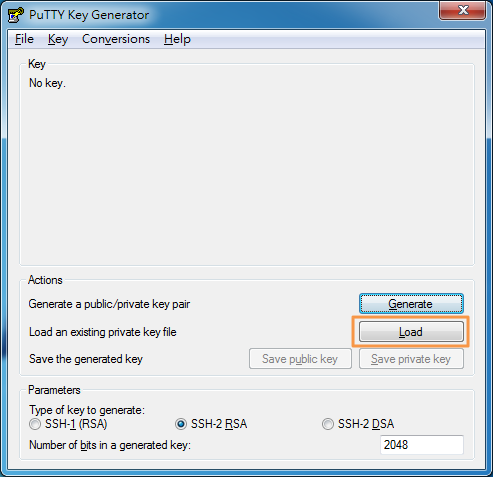
\includegraphics{openssh-putty-003.png}
\end{quote}
\begin{itemize}
\item {} 
首先選取存放ssh-key的資料夾,此時可能會發現什麼檔案都沒有,接著變更下方的副檔名篩選欄,將預設的『PuTTY Private Key Files』變更設定為『All Files』,就會出現檔案,選取要載入的私鑰後點選下方的『開啟』按鈕

\end{itemize}
\begin{quote}

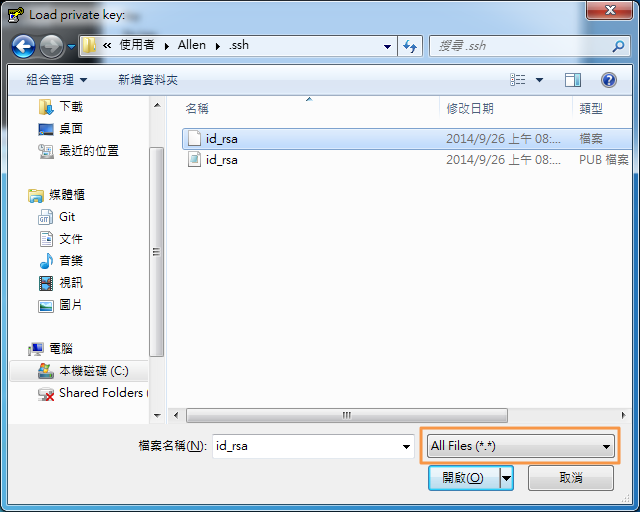
\includegraphics{openssh-putty-004.png}
\end{quote}
\begin{itemize}
\item {} 
開啟私鑰檔案後Pageant將會自動判斷到此檔為OpenSSH的格式,也有教學該如何轉換到Putty的格式

\end{itemize}
\begin{quote}

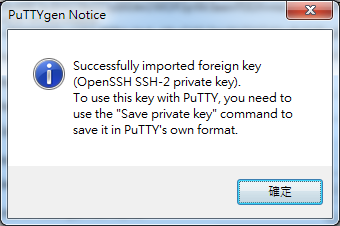
\includegraphics{openssh-putty-005.png}
\end{quote}
\begin{itemize}
\item {} 
點選『確認』關閉提示視窗後將會出現載入私鑰後的內容,依提示視窗所給的訊息,執行『Save private key』按鈕來儲存私鑰

\end{itemize}
\begin{quote}

\includegraphics{openssh-putty-006.png}
\end{quote}
\begin{itemize}
\item {} 
點選『Save private key』按鈕後會跳出存儲視窗,先選擇要存放的資料夾,接著在檔案名稱的地方輸入檔名,副檔名為『ppk』,最後點選存檔即可

\end{itemize}
\begin{quote}

\includegraphics{openssh-putty-007.png}
\end{quote}
\begin{itemize}
\item {} 
最後打開檔案管理員,找到存放ssh-key的資料夾,確認是否有完成存檔

\end{itemize}
\begin{quote}

\includegraphics{openssh-putty-008.png}
\end{quote}


\section{上傳公鑰(Public Key)}
\label{_doc/writing/index:public-key}
不論是用 {\hyperref[_doc/writing/index:ssh-key-puttygen]{\emph{Puttygen建立ssh-key}}}. 或是 {\hyperref[_doc/writing/index:ssh-key-gitbash]{\emph{Git Bash建立ssh-key}}}. 將私鑰留在要操作的電腦上,只要將公鑰,副檔名為pub的檔案寄給管理人員,請管理人員將公錀放到伺服器中設定後供使用者連線使用,檔案名稱格式參照 {\hyperref[_doc/writing/index:publickey-filename-format]{\emph{公鑰檔案名稱格式}}}.


\subsection{公鑰檔案名稱格式}
\label{_doc/writing/index:publickey-filename-format}\label{_doc/writing/index:id5}
使用者英文名字@單位名稱.pub


\section{存取檔案庫(Repo)}
\label{_doc/writing/index:repo}

\subsection{Pageant自動對應連線}
\label{_doc/writing/index:pageant}\begin{itemize}
\item {} 
啟動Pageant,打開『開始程式集』,找到 \textbf{TortoiseGit} 點選打開後就會看到如下圖的內容,點選執行『Pageant』

\end{itemize}
\begin{quote}

\includegraphics{pageant-001.png}
\end{quote}
\begin{itemize}
\item {} 
執行後可以在工作列右下角的找到如下圖的通知區域中是否有Pageant在運作中

\end{itemize}
\begin{quote}

\includegraphics{pageant-002.png}
\end{quote}
\begin{itemize}
\item {} 
點選該Pageant的圖示,將會出現『Pageant Key List』的視窗

\end{itemize}
\begin{quote}

\includegraphics{pageant-003.png}
\end{quote}
\begin{itemize}
\item {} 
點選『Add Key』後將會出現『Select Private Key File』的視窗,請找到存放私鑰的資料夾,選取副檔名為ppk的私鑰檔案,點選開啟

\end{itemize}
\begin{quote}

\includegraphics{pageant-004.png}
\end{quote}
\begin{itemize}
\item {} 
這樣就完成載入,如果電腦有需要連接不同的伺服器,可以重複上面的動作,加入N個私錀,Pageant將會自動對應

\end{itemize}
\begin{quote}

\includegraphics{pageant-005.png}
\end{quote}


\subsection{使用TortoiseGit Clone Repo}
\label{_doc/writing/index:tortoisegit-clone-repo}\begin{itemize}
\item {} 
當使用者的ssh-key建立好,伺服器上的設定也完成後,接下來就是將檔案庫(Repo)從伺服器上複製(clone)到操作電腦上,使用TortoiseGit軟體的圖形介面(GUI)去操作控制檔案庫(Repo),道先用開起檔案管理員,找到要建立檔案庫(Repo)的資料夾,然後在資料夾空白區塊點選滑鼠右鍵,就會有TortoiseGit的功能列選項可以使用,因為第一次存取檔案庫(Repo),所以要使用clone(中文版為:克隆)複製到本機操作電腦中。

\end{itemize}
\begin{quote}

\includegraphics{tortoisegit-clone-001.png}
\end{quote}
\begin{itemize}
\item {} 
點選右鍵功能列的『Git Clone...』或『Git 克隆...』後或出現設定視窗,在這邊最主要就是『URL』,目前的URL格式為『ssh://user@server/project.git』或『\href{mailto:user@server}{user@server}:project.git』,依URL格式轉換到目前伺服器的URL為『ssh://git@allen.go38.net/user2.git』或『\href{mailto:git@allen.go38.net}{git@allen.go38.net}:user2.git』,所以在視窗中的URL輸入正確的內容後,下方的目錄欄位會自動帶入project的名稱,此範例為user2,最後點選『確定』就開始執行複製(clone)

\end{itemize}
\begin{quote}

\textbf{英文版}

\includegraphics{tortoisegit-clone-002.png}

\textbf{中文版}

\includegraphics{tortoisegit-clone-003.png}
\end{quote}
\begin{itemize}
\item {} 
下圖為開始執行Git指令進度的視窗

\end{itemize}
\begin{quote}

\includegraphics{tortoisegit-clone-004.png}
\end{quote}
\begin{itemize}
\item {} 
在執行Git指令進度視窗的過程中,如果出現下圖的話有可能是Pageant沒有啟動,如果有啟動則要檢查一下私鑰是否有加入

\end{itemize}
\begin{quote}

\includegraphics{tortoisegit-clone-005.png}
\end{quote}
\begin{itemize}
\item {} 
下圖為Git指令執行成功的畫面

\end{itemize}
\begin{quote}

\includegraphics{tortoisegit-clone-006.png}
\end{quote}
\begin{itemize}
\item {} 
接下來再回來檔案管理員視窗看一下剛剛所複製(clone)的檔案庫(Repo)『user2』

\end{itemize}
\begin{quote}

\includegraphics{tortoisegit-clone-007.png}
\end{quote}


\subsection{使用TortoiseGit Push Repo}
\label{_doc/writing/index:tortoisegit-push-repo}\begin{itemize}
\item {} 
當文章內容修改完畢,要將檔案上傳推送(Push)到伺服器的檔案庫(Repo),只要在本機的檔案庫(Repo)資料夾中點選滑鼠右鍵的功能列中操作即可,在這個地方要注意一下,如果是對檔案庫(Repo)的資料夾上點選滑鼠右鍵操作Git指令這種方式是對整個檔案庫(Repo)操作,如果是在檔案庫(Repo)裡面的資料夾或檔案上點選滑鼠右鍵操作Git指令,這樣只會對該資料夾或檔案做處理,下圖就是在檔案庫(Repo)上執行Git指令的增加(Add),這個指令會將所有的檔案加入檔案庫(Repo)

\end{itemize}
\begin{quote}

\includegraphics{tortoisegit-push-001.png}
\end{quote}
\begin{itemize}
\item {} 
當點選增加(Add)後會出現一個視窗,該視窗內所列出的檔案就是與本機檔案庫(Repo)最後一個版本比對後尚未加入的檔案清單,在這邊可以選擇檔案要不要加入到檔案庫(Repo)中,可以自行勾選,如果檔案有很多想要全選或全部取消勾選,可在下面『全部選擇或取消』,最後點選『確定』

\end{itemize}
\begin{quote}

\includegraphics{tortoisegit-push-002.png}
\begin{itemize}
\item {} 
點選確定後,就會把所勾選的檔案加入到檔案庫(Repo)中,如果正常的狀況下,會出現所有的檔案都『已加入』,並且在最下面出現『完成』,這個時後並沒有將檔案上傳更新到伺服器,這些操作都還是在本機的檔案庫(Repo)中操作,接著點選如下圖中的提交(Commit)

\end{itemize}

\includegraphics{tortoisegit-push-003.png}
\end{quote}
\begin{itemize}
\item {} 
接著就會看到提交(Commit)的視窗,在視窗最上方的『記錄信息』填寫這次提交的簡略內容,方便之後尋找並回復,在下方可以勾選設定作者日期、設定作者,點選『加入Signed-off-by』會自動把設定作者的內容自動填到『記錄信息』的最下方,在『變動』可以看到這次提交(Commit)的檔案異動狀況,最後點選『確定』後就會把這次提交(Commit)的內容加入到檔案庫(Repo)

\end{itemize}
\begin{quote}

\includegraphics{tortoisegit-push-004.png}
\end{quote}
\begin{itemize}
\item {} 
點選『確定』後執行Git指令,這時就會出現『Git命令進度』的視窗,當看到『完成』後,本機的檔案庫(Repo)就把這次提交(Commit)的內容增加變更成最新的版本內容,但這時所有的操作還是都在本機的檔案庫(Repo)中操作,尚未上傳到遠端的伺服器中,如果要上傳推送(Push),請點選畫面中的『推送』

\end{itemize}
\begin{quote}

\includegraphics{tortoisegit-push-005.png}
\end{quote}
\begin{itemize}
\item {} 
點選『推送』後接著出現『推送』的設定視窗,在這邊先使用預設值,點選『確定』,開始將本機的檔案庫(Repo)上傳到遠端伺服器

\end{itemize}
\begin{quote}

\includegraphics{tortoisegit-push-006.png}
\end{quote}
\begin{itemize}
\item {} 
接著又會出現上傳推送(Push)指令進度視窗,此時就會開始上傳到遠端伺服器,最後會出現『完成』,這時就完成整個更新的流程

\end{itemize}
\begin{quote}

\includegraphics{tortoisegit-push-007.png}

\includegraphics{tortoisegit-push-008.png}
\end{quote}
\begin{itemize}
\item {} 
這時可以到 \href{http://allen.go38.net/cgi-bin/gitweb.cgi}{gitweb} 上看到該檔案庫(Repo)的更新內容

\end{itemize}
\begin{quote}

\includegraphics{tortoisegit-push-009.png}
\end{quote}


\subsection{使用Git Bash Clone Repo}
\label{_doc/writing/index:git-bash-clone-repo}\begin{itemize}
\item {} 
當使用者的ssh-key建立好,伺服器上的設定也完成後,接下來就是將檔案庫(Repo)從伺服器上複製(clone)到操作電腦上,使用Git 軟體的文字介面(console)去操作控制檔案庫(Repo),道先用開起檔案管理員,找到要建立檔案庫(Repo)的資料夾,然後在資料夾空白區塊點選滑鼠右鍵,就會有Git的功能列選項可以開啟Git Bash

\end{itemize}
\begin{quote}

\includegraphics{gitbash-clone-001.png}
\end{quote}
\begin{itemize}
\item {} 
在檔案管理員的資料夾下,使用滑鼠右鍵開啟Git Bash後也會一起切換到該資料夾目錄下

\end{itemize}
\begin{quote}

\includegraphics{gitbash-clone-002.png}
\end{quote}
\begin{itemize}
\item {} 
接著就輸入git clone指令將要存取的檔案庫(Repo)複製下來,依URL的格式輸入『git clone ssh://git@allen.go38.net/user2.git』或『git clone \href{mailto:git@allen.go38.net}{git@allen.go38.net}:user2.git』,正常無誤的話就會看到類似下圖的內容,接著執行『cd user2』切換到檔案庫user2,再使用『ls -al』列出該檔案庫(Repo)下的檔案內容

\end{itemize}
\begin{quote}

\includegraphics{gitbash-clone-003.png}
\end{quote}

使用Git Bash Push Repo
\begin{itemize}
\item {} 
在圖形介面的操作方式有介紹過如何使用TortoiseGit將寫好的文件上傳推送(Push)到伺服器上,現在使用 Git Bash文字指令的方式將寫好的文件上傳推送(Push)到伺服器上,操作的指令主要有三個,和TortoiseGit的操作是相同的;首先打開要處理的檔案庫(Repo),然後點選滑鼠右鍵,點選『Git Bash』,這時就會出現如下圖的視窗,操作的路徑會自動帶入

\end{itemize}
\begin{quote}

\includegraphics{gitBash-push-001.png}
\end{quote}
\begin{itemize}
\item {} 
操作如同TortoiseGit的『增加』,在Git下就是『git add .』後面的『.』就是全部都加入的意思,在在TortoiseGit會有好看的圖形介面可以使用勾選的方式選擇要不要加入,如果在Git Bash下只能用『git add filename』的方式去手動加入

\end{itemize}
\begin{quote}

\includegraphics{gitBash-push-002.png}
\end{quote}
\begin{itemize}
\item {} 
在這裡可以使用git status去顯示目前在本機檔案庫(Repo)內異動的狀況

\end{itemize}
\begin{quote}

\includegraphics{gitBash-push-003.png}
\end{quote}
\begin{itemize}
\item {} 
使提交(Commit)指令,『git commit -m ``記錄訊息''』,在使用Git提交一定要加入『記錄訊息』

\end{itemize}
\begin{quote}

\includegraphics{gitBash-push-004.png}
\end{quote}
\begin{itemize}
\item {} 
最後使用上傳推送(Push)指令將所提交(Push)的內容上傳到伺服器中,『git push』

\end{itemize}
\begin{quote}

\includegraphics{gitBash-push-005.png}
\end{quote}
\begin{itemize}
\item {} 
這時可以到 \href{http://allen.go38.net/cgi-bin/gitweb.cgi}{gitweb} 上看到該檔案庫(Repo)的更新內容

\end{itemize}
\begin{quote}

\includegraphics{gitBash-push-006.png}
\end{quote}


\section{GitWeb 線上觀看修改內容}
\label{_doc/writing/index:id7}
在伺服器上有安裝 \href{http://allen.go38.net/cgi-bin/gitweb.cgi}{gitweb} 此網站會將有開放的檔案庫(Repo)顯示在上面,下面有一些gitweb執行的畫面
\begin{itemize}
\item {} 
首頁 ,這裡會顯示所有檔案庫(Repo)的清單,後面會有一些連結可以不同的方式顯示記錄(summary \textbar{} shortlog \textbar{} log),檔案內容(tree)

\end{itemize}
\begin{quote}

\includegraphics{gitweb-001.png}
\end{quote}
\begin{itemize}
\item {} 
點選summary進入的頁面只會顯示比較近期的記錄,一樣後方也有一些連結,可以顯示commit的記錄,還有commitdiff與上一個版本的差異內容,snapshot可以打包下載這個版本的內容

\end{itemize}
\begin{quote}

\includegraphics{gitweb-002.png}
\end{quote}
\begin{itemize}
\item {} 
點選commit後會進詳細的內容,例如有幾個檔案新增、修改、刪除等,可點選diff去看該檔案的版本差異內容

\end{itemize}
\begin{quote}

\includegraphics{gitweb-003.png}
\end{quote}
\begin{itemize}
\item {} 
點選diff進入該檔案詳細的修改內容,如下圖,有『-』符號而且是紅色的文字代表被刪除,而有『+』符號並且是綠色文字代表新增內容,黑色文字就是沒有變動的內容

\end{itemize}
\begin{quote}

\includegraphics{gitweb-004.png}
\end{quote}
\begin{itemize}
\item {} 
在專案名稱下方有一些超連結可點選觀看,下面的圖片為點選『log』,會顯示比較完整的記錄項目

\end{itemize}
\begin{quote}

\includegraphics{gitweb-005.png}
\end{quote}
\begin{itemize}
\item {} 
點選『tree』會顯示該檔案庫(Repo)下所有的檔案內容,如果為檔案點選後可觀看檔案內容,若為資料夾則會進入該資料夾並顯示其檔案內容

\end{itemize}
\begin{quote}

\includegraphics{gitweb-006.png}
\end{quote}


\chapter{共筆寫作操作流程(GitHub)}
\label{_doc/writing/index-github::doc}\label{_doc/writing/index-github:github}
在上一版的「共同寫作操作流程」文件中是使用 \href{https://code.google.com/p/tortoisegit/}{TortoiseGit} 存取Git伺服器上的儲存庫(Repo),因為最後使用 \href{https://github.com/}{GitHub} 平台,所以這篇主要是說明如何透過GitHub的軟體「\href{https://windows.github.com/}{GitHub Windows}」共同存取寫作文件,當然也可以透過「\href{https://windows.github.com/}{GitHub Windows}」存取Go38 Git伺服器上的儲存庫(Repo),在「\href{https://windows.github.com/}{GitHub Windows} 」軟體的操作上非常的簡單,而且也會自動產生ssh-key,節省了很多的步驟,而且所產生的ssh-key也可以直接供Go38的Git伺服器所使用,而Go38伺服器上的儲存庫(Repo)也可以使用「\href{https://windows.github.com/}{GitHub Windows}」存取,下方的流程式為共筆寫作的流程圖。

\includegraphics{_doc/writing/pic/FlowChart.png}


\section{相關軟體安裝}
\label{_doc/writing/index-github:id5}

\subsection{GitHub Windows}
\label{_doc/writing/index-github:id6}\begin{itemize}
\item {} 
打開 \href{https://windows.github.com/}{GitHub Windows} 網站,首頁就有『Download GitHub for Windows』連結,點選此連結下載

\end{itemize}
\begin{quote}

\includegraphics{GitHub-Install-001.png}
\end{quote}
\begin{itemize}
\item {} 
下載完後執行安裝程式『GitHubSetup.exe』,如果電腦已經安裝過GitHub Windows,執行後會直接啟動GitHub Windows程式;若沒安裝過,執行後會檢查電腦所需要的元件,如下圖在第一次安裝由於電腦中沒有『Microsoft .NET Framework 4.5(x86 and x64)』這個元件,會要求安裝,點選下方的『Accept』即可

\end{itemize}
\begin{quote}

\includegraphics{GitHub-Install-002.png}

\includegraphics{GitHub-Install-003.png}
\end{quote}
\begin{itemize}
\item {} 
如果作業系統已安裝過『Microsoft .NET Framework 4.5(x86 and x64)』元件,執行後就直接出現GitHub安裝視窗,直接點選『Install』開始安裝

\end{itemize}
\begin{quote}

\includegraphics{GitHub-Install-004.png}
\end{quote}
\begin{itemize}
\item {} 
下圖為下載及安裝進度視窗,執行完就安裝成功

\end{itemize}
\begin{quote}

\includegraphics{GitHub-Install-005.png}
\end{quote}
\begin{itemize}
\item {} 
Connect,安裝完第一次執行GitHub Windows的畫面如下,輸入GitHub帳號及密碼,點選『Log in』登入與GitHub平台連線

\end{itemize}
\begin{quote}

\includegraphics{GitHub-Install-006.png}
\end{quote}
\begin{itemize}
\item {} 
Configue,設定git顯示的使用者名稱及E-Mail帳號,輸入完點選『Continue』

\end{itemize}
\begin{quote}

\includegraphics{GitHub-Install-007.png}
\end{quote}
\begin{itemize}
\item {} 
Repositories,這一步軟體會自動尋找本機的儲存庫(Repo),如果沒有找到,直接點選『dashboard』,進入軟體主畫面。

\end{itemize}
\begin{quote}

\includegraphics{GitHub-Install-008.png}
\end{quote}


\section{存取 Github Repo}
\label{_doc/writing/index-github:github-repo}

\subsection{複製Clone Repo}
\label{_doc/writing/index-github:clone-repo}\begin{itemize}
\item {} 
當安裝完GitHub Windows後,在還沒有複製(Clone)儲存庫(Repo)的狀況下,會看到如下面GitHub初始畫面,啟動後是很乾淨,什麼都沒有,只有在畫面中出現『Get started by adding a repository.』

\end{itemize}
\begin{quote}

\includegraphics{GitHub-Clone-001.png}
\end{quote}
\begin{itemize}
\item {} 
接下來點選左上角的『+』後會出現一個功能視窗,這個視窗主要的功能就是新增儲存庫(Repo),可以看到視窗最上方有兩個選項『Creat』和『Clone』, 下圖為『Create』的畫面,設定Name和Local path後,點選下方的『Create repository』,就可以在所選的本機資料夾路徑中建立一個新的Git儲存庫(Repo),最後可以使用Git Windows軟體發佈到GitHub平台所註冊的帳號中。

\end{itemize}
\begin{quote}

\includegraphics{GitHub-Clone-002.png}
\end{quote}
\begin{itemize}
\item {} 
下圖為『Clone』的畫面,當點選到『Clone』後,下方會自動載入安裝時所登入的GitHub帳號中所有的儲存庫(Repo)

\end{itemize}
\begin{quote}

\includegraphics{GitHub-Clone-003.png}
\end{quote}
\begin{itemize}
\item {} 
只要點選名稱,如『go38/MoodleBook』,再點選下方的『Clone repository』

\end{itemize}
\begin{quote}

\includegraphics{GitHub-Clone-004.png}
\end{quote}
\begin{itemize}
\item {} 
在複製(Clone)之前會出『瀏覽資料夾』的視窗,在此處點選儲存庫(Repo)要放在資料夾,如畫面中為預設的路徑(C:/Users/使用者名稱/我的文件/GitHub)

\end{itemize}
\begin{quote}

\includegraphics{GitHub-Clone-005.png}
\end{quote}
\begin{itemize}
\item {} 
確認資料夾後就會開始複製(Clone)到本機電腦,完成後會看到如下的畫面,畫面主要分為三個區塊,左邊為本機的儲存庫(Repo),如果有多個儲存庫(Repo)可點選做切換,而中間的『History』就是依左方所點選儲存庫(Repo)的歷史推送(Push)記錄,點選中間的歷史推送記錄後,在右方會顯示該次的異動內容,另外在『History』上方有個『master』,這為目前的分支(Branch)名稱,點選後可以切換分支或建立新的分支。

\end{itemize}
\begin{quote}

\includegraphics{GitHub-Clone-006.png}
\end{quote}


\subsection{檔案新增刪除修改}
\label{_doc/writing/index-github:id8}\begin{itemize}
\item {} 
把共筆的儲檔庫(Repo)複製(Clone)到本機資料夾中後就可以開始編寫內容,當想把編寫好的內容放到遠端時,如果是使用Git Shell文字模式的狀況下,需要自行輸入指令,如要把新增的檔案加到儲存庫(Repo)則輸入「git add .」,「git add filename」,若要把該檔案從儲存庫中刪除,使用「git rm filename」,那如果使用TortoiseGit軟體,也需要在該檔案點選右鍵去找到新增或刪除該檔案的功能選項,但使用GitHub Windows軟體,不需要在要新增或刪除的檔案去操作功能選項,也不需要自行下Git指令,只要打開GitHub Windows軟體,它會自動把檔案異動內容做處理並顯示在軟體中,如下圖的『Uncommitted changes』,將還沒有提交(Commit)前的異動內容顯示於此區塊。

\end{itemize}
\begin{quote}

\includegraphics{GitHub-Commit-001.png}
\end{quote}


\subsection{提交 Commit Repo}
\label{_doc/writing/index-github:commit-repo}\begin{itemize}
\item {} 
儲存庫(Repo)中的檔案異動完畢,可以點選『Show』,下方會出現摘要簡介(Summary)及說明(Description),至少要輸入摘要簡介(Summary)這個輸入欄位,讓其他編輯者了解此次提交(Commit)的目的,那如果要寫的比較詳細,請填寫說明(Description)的輸入欄位,如果在提交前想要看一下檔案的異動詳細內容,可在右方的區塊看到所列出的檔案,每個檔案都可以點選觀看該檔案的修改內容減號『-』代表刪除,加號『+』代表新增,填寫完並且確認完檔案後點選下方的『Commit to master』即可,「master」是分析的名稱。

上面的操作轉換到Git Shell文字模式下,需要輸入『git commit』,然後會自動在文字編輯器下開起一個檔案,需要在上面輸入這次提交(commit)的訊息,最後儲存檔案結束,如果要快一點的話可以用『git commit -m ``摘要簡介(Summary)''』即可,此外可以執行『git status』列出此次提交的檔安異動狀況。

\end{itemize}
\begin{quote}

\includegraphics{GitHub-Commit-002.png}
\end{quote}
\begin{itemize}
\item {} 
當點選『Commit to 分析名稱』後,『Uncommitted changes』的文字就會轉變成『Unsynced changes』,那右上方的『Sync』後方就會出現一個數字,該數字代表本機的儲存庫(Repo)執行了幾次的提交(Commit)動作,並且尚未推送(Push)到遠端伺服器中。下方有個『Undo』的按鈕,可以取消這一次的提交(Commit)動作。

\end{itemize}
\begin{quote}

\includegraphics{GitHub-Commit-003.png}
\end{quote}


\subsection{推送 Push Repo}
\label{_doc/writing/index-github:push-repo}\begin{itemize}
\item {} 
在軟體畫面右上方的『Sync』後方有數字出現,代表有提交(Commit)動作,而且尚未執行推送(Push),使用GitHub Windows執行推送(Push)也是非常的簡單,只要在『Sync』上點選一下,就會自動推送到遠端的伺服器中,完成推送(Push)後,『Unsynced changes』下的項目內容就會出現在『History』中,而且『Sync』後方的數字也會不見。

這個『Sync』的動作,在Git Shell文字模式下,就是輸入Git指令『git push』。

\end{itemize}
\begin{quote}

\includegraphics{GitHub-Commit-004.png}
\end{quote}


\section{存取 Go38 Git Repo}
\label{_doc/writing/index-github:go38-git-repo}
使用GitHub Windows存取GitHub平台的存取很簡單方便,因為GitHub Windows本來就是專為GitHub平台操作使用的軟體,那如果要操作其他Git伺服器的儲存庫(Repo),例如Go38伺服器上的Git儲存庫(Repo),要如何操作使用呢?以下會說明該如何操作,主要有幾個步驟和GitHub Widnwos不同,如下


\subsection{寄送公鑰(Public Key)}
\label{_doc/writing/index-github:public-key}\begin{itemize}
\item {} 
因為在安裝GitHub Windows軟體時,會自動產生一組公鑰「github\_rsa.pub」與私鑰「github\_rsa」在使用者家目錄下的「.ssh」資料夾中,打開「.ssh」資料夾,將公鑰「github\_rsa.pub」複製一份,然後變更檔案名稱,然後將該檔案傳送給Go38管理者,將會使用此公鑰建立使用者。

\end{itemize}
\begin{quote}

\includegraphics{GitHub-sshkey.png}
\end{quote}


\subsection{複製Clone Repo}
\label{_doc/writing/index-github:id9}\begin{itemize}
\item {} 
當使用者建立完成後要複製(Clone)Go38上的儲存庫(Repo),這裡的操作方式和GitHub平台不同,GitHub Windows可以直接使用GitHub的帳號登入並直接點複製(Clone),但這裡我們需要使用Git Shell的文字模式執行『git clone \href{mailto:git@allen.go38.net}{git@allen.go38.net}:MoodleBook.git』,將Go38上的MoodleBook儲存庫(Repo)複製(Clone)到本機電腦中,如下圖

\end{itemize}
\begin{quote}

\includegraphics{GitHub-Shell-001.png}
\end{quote}


\subsection{加入至GitHub Windows}
\label{_doc/writing/index-github:id10}
打開GitHub Windows軟體,怎麼看好像都沒有方法可以加入從別的伺服器中複製(Clone)下來的儲存庫(Repo),在這有找到兩種加入的方法,如下


\subsubsection{方法一:Scan for repositories}
\label{_doc/writing/index-github:scan-for-repositories}\begin{itemize}
\item {} 
點選GitHub Windows右上角的齒輪(tools and options),點選功能選單中的『Options...』

\end{itemize}
\begin{quote}

\includegraphics{GitHub-Option-001.png}
\end{quote}
\begin{itemize}
\item {} 
點選後會出現如下圖的Options視窗,尋找畫面中的放大鏡圖案『Scan for repositories』,並點選它

\end{itemize}
\begin{quote}

\includegraphics{GitHub-Option-002.png}
\end{quote}
\begin{itemize}
\item {} 
此時就會出現如下圖『Scan for repositories』的畫面,畫面中會出現在本機所找到的儲存庫(Repo),經過測試GitHub Windows只會找使用者家目錄「C:Users使用者名稱」以下的資料夾,如果是放在其他資料夾下沒辦法被自動搜尋到的儲存庫(Repo)可使用方法二加入。

\end{itemize}
\begin{quote}

\includegraphics{GitHub-AddOtherGit-001.png}
\end{quote}
\begin{itemize}
\item {} 
在本機電腦中可能有很多的儲存庫(Repo),如下圖就有找到兩個,預設都是勾選的,因為只要加入MoodleBook,所以把其他的儲存庫(Repo)取消勾選後,再點選下方的『Add』

\end{itemize}
\begin{quote}

\includegraphics{GitHub-AddOtherGit-002.png}
\end{quote}
\begin{itemize}
\item {} 
下圖為加入Go38的MoodleBook存儲庫(Repo)後的狀況,會發現所加入的MoodleBook存儲庫(Repo)會放在標籤『Other』下方,而GitHub的儲存庫會被歸類在『GitHub』標籤下

\end{itemize}
\begin{quote}

\includegraphics{GitHub-AddOtherGit-003.png}
\end{quote}


\subsubsection{方法二:拖曳資料夾}
\label{_doc/writing/index-github:id11}\begin{itemize}
\item {} 
第二種方法最簡單,只要打開檔案管理員,找到存放儲存庫(Repo)的資料夾,然後點選滑鼠左鍵不放,然後拉動拖曳儲存庫(Repo)的資料夾到GitHub Windows上,會看到出現『Drop to add repository』,然後放開滑鼠左鍵即可

\end{itemize}
\begin{quote}

\includegraphics{GitHub-DropToAdd-001.png}
\end{quote}
\begin{itemize}
\item {} 
接著看到MoodleBook已經被加入到『Other』標籤下

\end{itemize}
\begin{quote}

\includegraphics{GitHub-DropToAdd-002.png}
\end{quote}


\chapter{Ubuntu 安裝}
\label{_doc/ubuntu/index::doc}\label{_doc/ubuntu/index:ubuntu}

\chapter{軟體安裝}
\label{_doc/software/index::doc}\label{_doc/software/index:id1}\begin{itemize}
\item {} 
TortoiseGit 安裝

\item {} 
Git 安裝

\end{itemize}


\chapter{Indices and tables}
\label{index:indices-and-tables}\begin{itemize}
\item {} 
\emph{genindex}

\item {} 
\emph{modindex}

\item {} 
\emph{search}

\end{itemize}



\renewcommand{\indexname}{Index}
\printindex
\end{document}
